\chapter{Utilisation des programmes externes}
\label{chap-external-programs}
Ce chapitre présente l’utilisation des différents programmes qui composent Unitex. Ces
programmes, qui se trouvent dans le répertoire \verb+Unitex/App+, sont appelés automatiquement par
l'interface (en fait, \verb+UnitexToolLogger+ est appelé, afin de réduire de manière importante la taille du fichier zip).
Il est possible de voir les commandes qui ont été exécutées en cliquant sur  "Info>Console". Il est aussi possible de voir les options des differents programmes dans "Info>Help on commands" (voir Figure \ref{fig-help}). Remarquons que tous les programmes Unitex possèdent l'option \verb$-h$/\verb$--help$.

\bigskip
\begin{figure}[!h]
\begin{center}
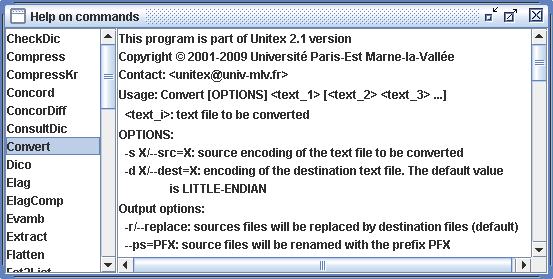
\includegraphics[width=14cm]{resources/img/fig11-1.png}
\caption{Help on commands\label{fig-help}}
\end{center}
\end{figure}

\bigskip
\noindent IMPORTANT: plusieurs programmes utilisent le répertoire du texte (\verb+mon_texte_snt+).
Ce répertoire est créé par l’interface graphique après la normalisation du texte. Si vous travaillez en ligne de commande, vous devrez créer ce répertoire vous-même après l’exécution du programme
\verb+Normalize+.\index{Répertoire!texte}

\bigskip
\noindent IMPORTANT (2): lorsqu’un paramètre contient des espaces, vous devez l’entourer de
guillemets pour qu’il ne soit pas considéré comme plusieurs paramètres.

\index{Texte!répertoire}\index{Programmes externes!\verb+Normalize+}\index{\verb+Normalize+}

\bigskip
\noindent ATTENTION (3): beaucoup de programmes utilisent un fichier \verb+Alphabet.txt+. Cette
information peut être omise pour l'ensemble de ces programmes. Dans ce cas, une définition (par
défaut) de lettres est utilisée (voir \verb+u_is_letter+ dans le fichier source\verb$Unicode.cpp$).


\section{Création de fichiers log}\index{Création de fichiers log}
\label{section-creating-log-files}

\bigskip
\begin{figure}[!h]
\begin{center}
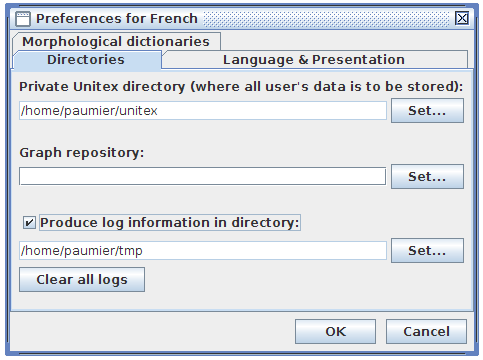
\includegraphics[width=10cm]{resources/img/fig11-1a.png}
\caption{Configuration de fichiers log\label{fig-logging-config}}
\end{center}
\end{figure}

Vous pouvez créer des fichiers \verb+log+ des programmes externes exécutés.
Ces fichiers log peuvent être utiles pour le débogage ou des tests de régression. Vous avez juste
besoin d'activer cette fonctionnalité dans le cadre Préférences. Vous devez simplement choisir un
répertoire de fichiers log dans lequel tous les fichiers sont stockés, et cocher la case "Produce
log"
En cliquant sur le bouton "Clear all logs" vous supprimez tous les fichiers log éventuellement
contenus dans ce répertoire. Désormais, toute nouvelle exécution du promme produit un fichier
\verb+unitex_log_XXX.ulp+ dans le répertoire de fichiers log. \verb+XXX+ représente le numéro de
log qui se trouve dans la console (voir section suivante).



\section{La console}\index{Console}
\label{section-console}
Lorsque Unitex lance un programme externe, la ligne de commande appelée est mémorisée dans la
console. Pour la voir, cliquez sur Info ``> Console''. Quand une commande n'émet aucun message
d'erreur, elle est affichée avec une icône verte. Sinon, l'icône est un triangle rouge sur lequel
vous pouvez cliquer pour voir les messages d'erreur, comme indiqué sur la figure \ref{fig-console}
. Ceci est utile lorsque un message d'erreur se produit si vite que vous ne pouvez pas le lire. Si
une commande a été enregistrée, son numéro de log apparaît dans la deuxième colonne. Notez que vous
pouvez exporter toutes les commandes affichées dans la console vers le presse-papiers avec Ctrl + C.

\bigskip
\begin{figure}[!h]
\begin{center}
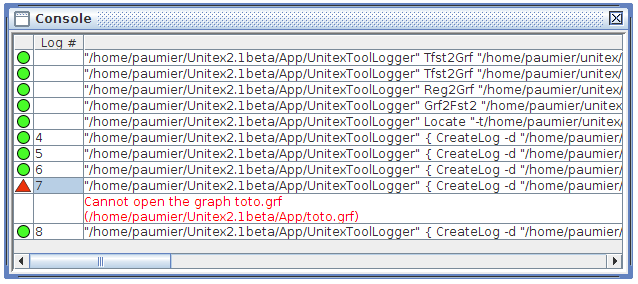
\includegraphics[width=15cm]{resources/img/fig11-2.png}
\caption{Console\label{fig-console}}
\end{center}
\end{figure}

\section{Unitex JNI}
\index{Unitex JNI}
\label{section-unitex-JNI}

Vous pouvez utilisez Unitex avec JNI by en incluant les imports suivants : 
\begin{verbatim}
import fr.umlv.unitex.jni.UnitexJni;
import java.io.*;
import fr.umlv.unitex.*;
\end{verbatim}
Ceci vous permet de charger en mémoire les dictionnaires (.bin), les grammaires ou graphes dictionnaires (.fst2) et les fichiers alphabet et de les garder en mémoire de manière persistante. Vous utilisez alors le nom de fichier renvoyé par la foncton loadPersistent*.

\begin{verbatim}
String persistentAlphabet = UnitexJni.loadPersistentAlphabet("/.../unitex/French/Alphabet.txt");
String persistentFst2 = UnitexJni.loadPersistentFst2("/.../unitex/French/Dela/fogg-r.fst2");
String persistentDictionary = UnitexJni.loadPersistentDictionary(
		"/.../unitex/French/Dela/communesFR+.bin");
\end{verbatim}


\section{Paramètres de codage des fichiers textes}\index{Paramètres de codage des fichiers textes}\index{Fichier!texte!paramètres de codage}
\label{section-text-file-encoding-parameters}
Unitex utilise Unicode pour les fichiers textes \ref{unicode-encoding}. Tous les programmes qui
lisent ou écrivent des fichiers textes partagent les mêmes paramètres d'encodage. Les formats
possibles sont utf16le-bom, utf16le-no-bom, utf16be-bom, utf16be-no-bom, utf8-bom, utf8-no-bom, qui
correspondent à Unicode Big-Endian, Little-Endian et UTF-8, avec ou sans "Unicode byte order mark"
(bom) au début du fichier. Pour le format d'entrée, vous pouvez spécifier plusieurs encodages *-bom
(avec bom) codage séparées par des virgules, mais seulement un encodage *-no-bom (sans bom).

\bigskip
\noindent \textbf{OPTIONS:}
\begin{itemize}
\item \verb+-k=ENCODING+/\verb+--input_encoding=ENCODING+: format du texte source. Peut contenir
plusieurs valeurs séparées par des virgules;
\item \verb+-q=ENCODING+/\verb+--output_encoding=ENCODING+: format du texte de sortie. 
\end{itemize}

\noindent Par défaut, les valeurs sont: \verb+--input_encoding=utf16le-bom,utf16be-bom,utf8-bom+
\newline \verb+--output_encoding=utf16le-bom+.


\section{BuildKrMwuDic}\index{Programmes externes!\verb+BuildKrMwuDic+}\index{\verb+BuildKrMwuDic+}
\index{Génération du dictionnaire des mots composés coréens}\index{Dictionnaire!mots composés
coréens}
\verb+BuildKrMwuDic [OPTIONS] dic+

\bigskip
\noindent Ce programme génère des graphes de flexion pour les mots composés à partir d'un tableau
\verb+dic+ qui décrit chaque constituant de chaque mot composé
\bigskip
\noindent \textbf{OPTIONS:}
\begin{itemize}
\item \verb+-o GRF+/\verb+--output=GRF+: fichier \verb+.grf+ à produire;
\item \verb+-d DIR+/\verb+--directory=DIR+: répertoire de flexion qui contient les graphes de
	flexion nécéssaires pour produire les variantes morphologiques des racines;
\item \verb+-a ALPH+/\verb+--alphabet=ALPH+: fichier alphabet à utiliser;
\item \verb+-b BIN+/\verb+--binary=BIN+:  dictionnaire des mots simples de type \verb+.bin+ à
	utiliser;
\end{itemize}






\section{Cassys}\index{Programmes externes!\verb+Cassys+}\index{\verb+Cassys+}
\index{Cascade de transducteurs}
\verb+Cassys [OPTIONS] <snt>+

\bigskip
\noindent Ce programme applique une liste ordonnée de grammaires à un texte et construit un index
des occurrences trouvées.
\bigskip
\noindent \textbf{OPTIONS:}
\begin{itemize}
\item \verb+-a ALPH+/\verb+--alphabet=ALPH+: fichier alphabet de la langue;
\item \verb+-r X+/\verb+--transducer_dir=X+: prend un transducteur dans le répertoire \verb+X+ (ainsi ne
		donnez pas le chemin complet pour chaque transducteur; remarquons que \verb+X+ doit se
		terminer par un antislash;
	\item \verb+-w DIC/--morpho=DIC+: indique que \verb+DIC+ est un \verb+.bin+ dictionnaire à utiliser en mode morphologique.
		Utiliser autant de  \verb+-m XXX+ qu'il y a de \verb+.bin+. Vou pouvez égalemnt séparer plusieurs \verb+.bin+ par des deux-points.

\item \verb+-l TRANSDUCERS_LIST+/\verb+--transducers_list=TRANSDUCERS_LIST+: fichier
		contenant la liste des transducteurs avec leur mode d'application;
\item \verb+-s transducer.fst2+/\verb+--transducer_file=transducer.fst2+: un transducteur à
		appliquer;
\item \verb+-m output_policy+/\verb+--transducer_policy=output_policy+: le mode
		d'application du transducteur spécifié;
\item \verb+-t TXT+/\verb+--text=TXT+: le fichier texte avec l'extension \verb+.snt+ à modifier;
\item \verb+-i+/\verb+--in_place+: sigifie qu'il faut utiliser les mêmes répertoires \verb+csc/snt+
	pour chaque transducteur;
\item \verb+-d+/\verb+--no_create_directory+: signifie que tous les répertoires \verb+snt/csc+
	existent déjà et n'ont pas besoin d'être crées;
\item \verb+-g minus+/\verb+--negation_operator=minus+: utilise \verb+moins+ comme opérateur de
	négation pour les graphes version Unitex 2.0;
\item \verb+-g tilde+/\verb+--negation_operator=tilde+: utilise \verb+tilde+ comme opérateur de
	négation (par défaut);
\item \verb+-h+/\verb+--help+: affiche cette aide
\end{itemize} 	


\bigskip
\noindent Cassys applique une liste de grammaires à un texte et sauve les séquences reconnues dans
un fichier index nommé \verb+concord.ind+ stocké dans le répertoire texte.
Le fichier cible doit être un fichier snt avec son répertoire \verb+\_snt/+. 
Le fichier contenant la liste des transducteurs est un fichier dans lequel chaque ligne contient le
nom complet du transducteur suivi de son mode d'application.

\bigskip
\noindent A la place d'une liste, vous pouvez spécifier chaque fichier et mode d'application par un
ensemble de couple d'arguments pour représenter la liste \verb+-s/--transducer\_file+ et
\verb+-m/--transducer\_policy+ 
      
\bigskip
\noindent Le mode d'application peut être MERGE ou REPLACE.
      
\bigskip
\noindent L'option de fichier, l'option alphabet et l'option fichier liste de transducteurs sont
obligatoires
     
\bigskip
\noindent Comme le programme Locate, ce programme enregistre les références des occurrences dans un
fichier \verb+concord.ind+ stocké dans le répertoire \verb+\_snt\verb+ du texte.
Le fichier \verb+concord.ind+ produit est dans le même format que celui décrit chapitre
\ref{chap-file-formats} , mais la cascade peut être formée de graphes appliqués en mode merge ou
replace, de ce fait \#M ou \#R à la première ligne du fichier \verb+concord.ind+ n'a pas de sens dans ce contexte.



\section{CheckDic}\index{Programmes externes!\verb+CheckDic+}\index{\verb+CheckDic+}
\index{Vérification du format d'un dictionnaire}\index{Dictionnaire!vérification}
\verb+CheckDic [OPTIONS] dic+

\bigskip
\noindent Ce programme effectue la vérification du format d’un dictionnaire de type DELAS ou
DELAF.\verb+dic+ qui correspond au nom du dictionnaire à vérifier

\bigskip
\noindent \textbf{OPTIONS:}
\begin{itemize}
\item \verb+-f+/\verb+--delaf+: vérifie un dictionnaire de formes fléchies;
\item \verb+-s+/\verb+--delas+: vérifie un dictionnaire de formes canoniques;
\item \verb+-r+/\verb+--strict+: vérification stricte de la syntaxe, la déspécialisation des points
	et virgules;
\item \verb+-t+/\verb+--tolerate+: tolère des points et des virgules non déspécialisés (par défaut);
\item \verb+-n+/\verb+--no_space_warning+: tolère des espaces dans les codes
	grammaticaux/sémantiques/flexionnels;
\item \verb+-p+/\verb+--skip_path+: n'affiche pas le chemin complet du dictionnaire (utiles pour la
		compatibilité de fichiers de log sur plusieurs systèmes);
\item \verb+-a ALPH+/\verb+--alphabet=ALPH+: indique le fichier alphabet à utiliser. 
\end{itemize}

\bigskip
\noindent Le programme teste la syntaxe des lignes du dictionnaire. Il dresse également la liste des
caractères présents dans les formes fléchies et canoniques, la liste des codes grammaticaux
et syntaxiques ainsi que la liste des codes flexionnels utilisés. Les résultats de la vérification
sont stockés dans un fichier nommé \verb+CHECK_DIC.TXT+.\index{Fichier!\verb+CHECK_DIC.TXT+}

\bigskip
\noindent Le choix de \verb+--strict+ permet de détecter l'utilisation de points non déspécialisés
dans la forme fléchie ou de virgules non déspécialisées dans la forme canonique. L'option
\verb+--tolerate+ se comporte comme dans les versions Unitex 2.0 et antérieures et ne les détecte
pas.





\section{Compress}\index{Programmes externes!\verb+Compress+}\index{\verb+Compress+}
\index{Compression des dictionnaires}
\label{section-compress}
\verb+Compress [OPTIONS] dictionary+
\index{Dictionnaire!DELAF}\index{Dictionnaire!compression}
\index{Fichier!\verb+.dic+}\index{Fichier!\verb+.bin+}\index{Fichier!\verb+.inf+}

\bigskip
\noindent \textbf{OPTIONS:}
\begin{itemize}
\item \verb+-o BIN+/\verb+--output=BIN+: définit le fichier de sortie. Par défaut, un fichier
	\verb+xxx.dic+ produit un fichier \verb+xxx.bin+;
\item \verb+-f+/\verb+--flip+: indique que les formes fléchies et canoniques doivent être inversées
dans le dictionnaire comprimé. Cette option est utilisée pour construire un dictionnaire inversé
nécessaire au programme \verb+Reconstrucao+;
\item \verb+-s+/\verb+--semitic+: indique que l'algorithme de compression pour langue sémitique doit
être utilisé. Cette option utilisée avec des langues sémitiques comme l'arabe réduit sensiblement la
taille du dictionnaire produit;
\item \verb+--v1+: produit un fichier \verb+.bin+ ancienne manière;
\item \verb+--v2+: produit un fichier \verb+.bin+ nouvelle manière, mieux comprimé et sans
	limitation de taille de fichier à 16 Mb (par défaut)
\end{itemize}

\bigskip
\noindent Ce programme prend en paramètre un dictionnaire DELAF et le compresse.

La compression d’un dictionnaire \verb+dico.dic+ produit deux fichiers:
\begin{itemize}
  \item \verb+dico.bin+: fichier binaire contenant l’automate minimal des formes fléchies du
  	  dictionnaire ;
  \item \verb+dico.inf+: fichier texte contenant des formes comprimées permettant de reconstruire
les lignes du dictionnaire à partir des formes fléchies contenues dans l’automate.
\end{itemize}

\bigskip
\noindent Pour plus de détails sur les formats de ces fichiers, voir chapitre
\ref{chap-file-formats}.






\section{Concord}\index{Programmes externes!\verb+Concord+}\index{\verb+Concord+}\index{Concordance}
\label{section-Concord}
\index{Texte!modification}\index{Modification du texte}
\verb+Concord [OPTIONS] <index>+

\bigskip
\noindent Ce programme prend en paramètre un fichier d’index de concordance produit par le
programme \verb+Locate+ et produit une concordance. Il peut également produire une version
du texte modifiée prenant en compte les transductions associées aux occurrences. Voici la
description des paramètres:


\bigskip
\noindent \textbf{OPTIONS:}
\begin{itemize}
  \item \verb+-f FONT+/\verb+--font=FONT+: nom de la police de caractères à utiliser si la
  	  sortie est fichier HTML;
  \item \verb+-s N+/\verb+--fontsize=N+: taille de la police si la sortie est fichier HTML.
  	Les paramètres concernant la police sont ignorés si la sortie n’est pas au format HTML;
  \item \verb+--only_ambiguous+: Affiche seulement les occurrences identiques avec une sortie
  	  ambiguë, dans l'odre du texte.
  \item \verb+--only_matches+: cette option définit un mode sans contexte.
	En outre si elle est utilisée avec \verb+-t/--text+, Concord n'entoure pas les séquences
	reconnues de tabulations
  \item \verb+-l X+/\verb+--left=X+: nombre de caractères à gauche des occurrences (par défaut=0).
  	  Dans le mode Thai, ceci correspond au nombre de caractères non
  	  diacritiques.\index{Contexte!concordance}
  \item \verb+-r X+/\verb+--right=X+: nombre de caractères (non diacritiques dans le mode Thai)
	à droite des occurrences (par défaut=0). Si l'occurrence est plus petite que cette valeur,
	la ligne de concordance est complétée jusqu'à \verb+right+. Si l'occurrence est plus longue
	que la valeur définie par \verb+right+, elle est néanmoins entièrement conservée.
  
  \bigskip
  NOTE: Pour \verb+--left+ et \verb+--right+, vous pouvez ajouter le caractère \verb+s+
  pour arrêter au premier symbole de fin de phrase \verb+{S}+. Par exemple, si vous mettez 
  \verb+40s+ comme valeur de gauche, le contexte gauche sera au plus à 40 caractères, moins si le \verb+{S}+ est trouvé avant.
\end{itemize}

\bigskip
\noindent \textbf{Options de tri:}\index{Tri!de concordance}
\begin{itemize}
  \item \verb+--TO+: ordre dans lequel les occurrences apparaissent dans le texte (par défaut);
  \item \verb+--LC+: contexte gauche comme premier tri, occurrence comme second tri;
  \item \verb+--LR+: contexte gauche, contexte droit;
  \item \verb+--CL+: occurrence, contexte gauche;
  \item \verb+--CR+: occurrence, contexte droit;
  \item \verb+--RL+: contexte droit, contexte gauche;
  \item \verb+--RC+: contexte droit, occurrence.
\end{itemize}
\noindent Pour plus de détails sur ces modes de tri, voir la section
\ref{section-display-occurrences}.

\bigskip
\noindent \textbf{Options de sortie:}
\begin{itemize}
  \item \verb+-H+/\verb+--html+: produit une concordance au format HTML codée en UTF-8;
  	  \index{UTF-8} (par défaut);
  \item \verb+-t+/\verb+--text+: produit une concordance au format texte Unicode; 
  \item \verb+-g SCRIPT+/\verb+--glossanet=SCRIPT+: produit une concordance pour GlossaNet
  	  au format HTML. Le fichier HTML produit est codé en UTF-8;\index{GlossaNet}
  \item \verb+-p SCRIPT+/\verb+--script=SCRIPT+: produit une concordance au format HTML où les
  	  occurrences sont liens décrits par \verb+SCRIPT+. Par exemple, si vous utilisez
  	  
  \verb$-phttp://www.google.com/search?q=$, vous obtiendrez 
  une concordance au format HTML où les occurrences sont des liens vers des requêtes Google;

\item \verb+-i+/\verb+--index+: produit un index de la concordance, qui comporte
	les occurrences (avec les sorties des grammaires, s'il y en a), précédées par
	les positions des occurrences, dans le fichier texte, exprimées en caractères;
\item \verb+-u+ \verb+offsets+/\verb+--uima=offsets+: produit un index de la concordance relatif
	fichier texte original, avant toute opération effectuée par Unitex. Offsets 
	est le fichier produit par Tokenize avec l'option \verb+--output_offsets+
%  the same as \verb+--index+, but the ending position of each occurrence is also given;
\item \verb+-e+/\verb+--xml+: produit un index xml de la concordance;
\item \verb+-w+/\verb+--xml-with-header+: produit un index xml de la concordance avec une en-tête
	xml complète;
\item \verb+--lemmatize+: produit un fichier de concordance HTML spécial utilisé par l'interface de lemmatisation
	de l'interface graphique d'Unitex.


	REMARQUE:  les options -e et -w acceptent toutes deux un fichier d'offset, comme l'accepte -u 
\item \verb+--PRLG=X,Y+: produit une concordance pour des corpus PRLG où chaque ligne
	est préfixée par l'information extraite avec l'option \verb+--PRLG+ de Unxmlize. X est le
	fichier produit par l'option \verb+--PRLG+ de Unxmlize et Y est le fichier produit par
	l'option \verb+--output_offsets+ de Tokenize. Remarquons que si cette option est utilisée en
	plus avec \verb+-u+, l'argument Y remplace l'argument de \verb+-u+;
	
\item \verb+-A+/\verb+--axis+: presque pareil que \verb+--index+, mais les nombres
	représentent le caractère médian de chaque occurrence. Pour plus d'information,
	consultez \cite{axis};
\item \verb+-x+/\verb+--xalign+: un autre fichier index, utilisé par le module d'alignement de
	texte.
	Chaque ligne est formée de 3 entiers $X$ $Y$ $Z$ suivi du contenu de l'occurrence.
	$X$ est numéro de la phrase, partant de 1. $Y$ et $Z$ sont les positions de début et de fin
	de l'occurrence dans la phrase exprimée en caractères;
\item \verb+-m TXT+/\verb+--merge=TXT+: indique au programme qu'il doit produire une version
	modifiée du texte et l'enregistrer dans le fichier dénommé
	\verb+TXT+ (voir section \ref{section-modifying-text}).
	
\item  \verb+T--export_csv+: produit un fichier avec le séparateur tabulation export.csv dans l'ordre du texte avec le 
	format suivant:
	\subitem A B C D E F, où:
	\subitem  A=nombre de lignes dans le fichier .csv
	\subitem  B=nombre de phrases
	\subitem  C= référence PRLG, si elle existe
	\subitem  D=la forme fléchie présente dans le texte
	\subitem  E=le lemme, s'il existe
	\subitem  F=les codes, s'il y en a\\
	Pour fonctionner, cette option doit re appelée pour des fichier concord.ind, qui ne contiennent pas de token
	{S} ni espace
\end{itemize}

\bigskip
\noindent \textbf{Autres options:}
\begin{itemize}
\item \verb+-d DIR+/\verb+--directory=DIR+: indique au programme qu'il ne doit pas travailler avec
	le même répertoire que \verb+<index>+ mais avec \verb+DIR+;
  \item \verb+-a ALPH+/\verb+--alphabet=ALPH+: fichier alphabet utilisé pour le tri;
  \item \verb+-T+/\verb+--thai+: option à utiliser pour les concordances en Thai.
  \index{Alphabet}\index{Fichier!alphabet}
\end{itemize}

\index{Fichier!\verb+.html+}\index{Fichier!\verb+.txt+}
\bigskip
\noindent Le résultat de l’application de ce programme est un fichier \verb+concord.txt+
si la concordance a été construite en mode texte, un fichier \verb+concord.html+ pour les modes
 \verb+--html+, \verb+--glossanet+ ou \verb$--script$, et un fichier texte dont le nom a été
défini par l’utilisateur si le programme a construit une version modifiée du texte.


\bigskip
\noindent En mode \verb+--html+, l’occurrence est codée comme un lien. La référence associée à ce
lien est de la forme \verb+<a href="X Y Z">+. \verb+X+ et \verb+Y+ représentent les positions de
début et de fin de l’occurrence en caractères dans le fichier \verb+text_name.snt+. \verb+Z+
représente le numéro de la phrase dans laquelle apparaît l’occurrence.







\section{ConcorDiff}\index{Programmes externes!\verb+ConcorDiff+}\index{\verb+ConcorDiff+}
\verb+ConcorDiff [OPTIONS] <concor1> <concor2>+

\bigskip
\noindent Ce programme prend deux fichiers de concordance et produit une page HTML montrant les
différences entre ces deux concordances (voir section
\ref{section-comparing-concordances}, page \pageref{section-comparing-concordances}). 
\verb+<concor1>+ et \verb+<concor2>+ fichiers de concordances (.ind) doivent avoir des noms  
absolus, car Unitex en déduit le texte sur lequel elles ont été calculées;

\bigskip
\noindent \textbf{OPTIONS:}
\begin{itemize}
  \item \verb+-o X+/\verb+--out=X+: page HTML de sortie;
  \item \verb+-f FONT+/\verb+--font=FONT+: police à utiliser dans le page HTML de sortie;
  \item \verb+-s N+/\verb+--size=N+: taille de police à utiliser dans le page HTML de sortie;
  \item \verb+-d/--diff_only+: ne pas afficher les séquences identiques;
\end{itemize}







\section{Convert}\index{Programmes externes!\verb+Convert+}\index{\verb+Convert+}
\verb+Convert [OPTIONS] <text_1> [<text_2> <text_3> ...]+

\index{Unicode}
\bigskip
\noindent Ce programme permet de transcoder des fichiers textes.

\bigskip
\noindent \textbf{OPTIONS:}
\begin{itemize}
\item \verb+-s X+/\verb+--src=X+: encodage d'entrée;
\item \verb+-d X+/\verb+--dest=X+: encodage de sortie
	(par défaut=\verb$LITTLE-ENDIAN$);
\end{itemize}

\bigskip
\noindent \textbf{Options de translitération (seulement pour l'arabe):}
\begin{itemize}
\item \verb+-F+/\verb+--delaf+: l'entrée est un DELAF et l'on veut seulement translitérer les formes
	fléchies et canoniques;
\item \verb+-S+/\verb+--delas+: l'entrée est un DELAS et l'on veut seulement translitérer les formes
	canoniques.
\end{itemize}


\bigskip
\noindent \textbf{Options de sortie:}
\begin{itemize}
\item \verb+-r+/\verb+--replace+: la conversion écrase les fichiers source (par défaut);
\item \verb+-o file+/\verb+--output=file+: nom du fichier de destination (seulement un fichier à convertir);
\item \verb+--ps=PFX+: les fichiers sources sont renommés avec le préfixe \verb+PFX+;
        (\verb+toto.txt+ $\Rightarrow$ \verb+PFXtoto.txt+);
\item \verb+--pd=PFX+: les fichiers destinations sont renommés avec le préfixe \verb+PFX+;
\item \verb+--ss=SFX+: les fichiers sources sont renommés avec le suffixe \verb+SFX+;
        (\verb+toto.txt+ $\Rightarrow$ \verb+totoSFX.txt+);
\item \verb+--sd=SFX+: les fichiers destinations sont renommés avec le suffixe \verb+SFX+.
\end{itemize}

\bigskip
\noindent \textbf{Options HTML:}

\noindent \verb+Convert+ offre des options spéciales pour les fichiers HTML. Vous pouvez utiliser  une combinaison des options suivantes:

\begin{itemize}
\item \verb+--dnc+ (Decode Normal Chars): des séquences comme \verb+&eacute;+
	\verb+&#120;+ et \verb+&#xF8;+ sont décodées comme un unique caractère
	unicode, sauf si elles representent un caractère de contrôle HTML;
  
  \item \verb+--dcc+ (Decode Control Chars): \verb+&lt;+ \verb+&gt;+
  	  \verb+&amp;+ et \verb+&quot;+ sont décodés comme \verb+<+ \verb+>+
  \verb+&+ et les quote (de même pour leur représentation  décimales et hexadécimales);
  
  \item \verb+--eac+ (Encode All Chars): chaque caractère non supporté par l'encodage de sortie
  	  est représenté par une chaîne comme \verb+&#457;+
  
  \item \verb+--ecc+ (Encode Control Chars): \verb+<+ \verb+>+
  	  \verb+&+ et les  quote sont encodés par \verb+&lt;+ \verb+&gt;+
  	  \verb+&amp;+ et \verb+&quot;+
\end{itemize} 

\noindent Par défaut, toutes les options HTML sont désactivées.

\bigskip
\noindent \textbf{Autres options:}
\begin{itemize}
\item \verb+-m+/\verb+--main-names+: imprime la liste des noms principaux des encodage;
\item \verb+-a+/\verb+--aliases+: imprime la liste des alias d'encodage;
\item \verb+-A+/\verb+--all-infos+: imprime toutes les information concernant tous les encodages;
\item \verb+-i X+/\verb+--info=X+: imprime toutes les information concernant l'encodage X.
\end{itemize}

\bigskip
\noindent Les encodages prennent leurs valeurs dans la liste suivante  (liste non exhaustive, voir
	ci-dessous):

\bigskip
\verb$FRENCH$

\verb$ENGLISH$

\verb$GREEK$

\verb$THAI$

\verb$CZECH$

\verb$GERMAN$

\verb$SPANISH$

\verb$PORTUGUESE$

\verb$ITALIAN$

\verb$NORWEGIAN$

\verb$LATIN$ (default latin code page)

\verb$windows-1252$: Microsoft Windows 1252 - Latin I (Western Europe \& USA)

\verb$windows-1250$: Microsoft Windows 1250 - Central Europe

\verb$windows-1257$: Microsoft Windows 1257 - Baltic

\verb$windows-1251$: Microsoft Windows 1251 - Cyrillic

\verb$windows-1254$: Microsoft Windows 1254 - Turkish

\verb$windows-1258$: Microsoft Windows 1258 - Viet Nam

\verb$iso-8859-1  $: ISO 8859-1  - Latin 1 (Europe de l'ouest \& USA)

\verb$iso-8859-15 $: ISO 8859-15 - Latin 9 (Western Europe \& USA)

\verb$iso-8859-2  $: ISO 8859-2  - Latin 2 (Eastern and Central Europe)

\verb$iso-8859-3  $: ISO 8859-3  - Latin 3 (Southern Europe)

\verb$iso-8859-4  $: ISO 8859-4  - Latin 4 (Northern Europe)

\verb$iso-8859-5  $: ISO 8859-5  - Cyrillic

\verb$iso-8859-7  $: ISO 8859-7  - Greek

\verb$iso-8859-9  $: ISO 8859-9  - Latin 5 (Turkish)

\verb$iso-8859-10 $: ISO 8859-10 - Latin 6 (Nordic)

\verb$next-step   $: NextStep code page

\verb$LITTLE-ENDIAN$

\verb$BIG-ENDIAN$

\verb$UTF8$







\section{Dico}\index{Programmes externes!\verb+Dico+}\index{\verb+Dico+}
\index{Dictionnaire!application}
\verb+Dico [OPTIONS] <dic_1> [<dic_2> <dic_3>...]+

\bigskip
\noindent Ce programme applique des dictionnaires à un texte. Le texte doit avoir été découpé en
unités lexicales par le programme \verb+Tokenize+.

\bigskip
\noindent \textbf{OPTIONS:}
\begin{itemize}
\item \verb+-t TXT+/\verb+--text=TXT+: nom complet du fichier texte \verb+.snt+;
\item \verb+-a ALPH+/\verb+--alphabet=ALPH+: le fichier alphabet à utiliser;
\item \verb+-m DICS+/\verb+--morpho=DICS+: ce paramètre optionnel liste
	les dictionnaires du mode morphologique, si la présence de dictionnaires
	\verb+.fst2+ rend cette information nécessaire. \verb+DICS+ représente une liste de fichiers \verb+.bin+ (avec leur nom
		complet) séparés par des points-virgules;
\item \verb+-K+/\verb+--korean+: indique à \verb$Dico$ qu'il travaille sur du coréen;
\item \verb+-s+/\verb+--semitic+: indique à \verb$Dico$ qu'il travaille sur une langue sémitique
	(nécessaire  si \verb$Dico$ doit compresser un dictionnaire);
\item \verb+-u X+/\verb+--arabic_rules=X+: désigne le fichier de configuration des règles
	typographiques de l'arabe;.
\item \verb+r X+/\verb+--raw=X+: indique que \verb$Dico$ devrait simplement produire un fichier de
	sortie X contenant les mots simples et composés, sans exiger un répertoire texte. Si X est
	omis, les résultats sont affichés sur la sortie standard.
\end{itemize}

\bigskip
\noindent \verb+<dic_i>+ représente le chemin d’accès complet à un dictionnaire. Le dictionnaire
doit être soit un dictionnaire compressé au format \verb+.bin+ (obtenu avec le programme
	\verb+Compress+) soit un graphe dictionnaire au format\verb+.fst2+ (voir section
\ref{section-applying-dictionaries}, page \pageref{section-applying-dictionaries}).
	\index{Fichier!\verb+.bin+} Il est possible de donner des priorités aux dictionnaires. Pour
	les détails voir section \ref{section-dictionary-priorities}.

\bigskip
\noindent Le programme \verb+Dico+ produit les fichiers suivants et les sauve dans le répertoire du
texte

\begin{itemize}
  \index{Fichier!\verb+dlf+}\index{Fichier!\verb+dlc+}\index{Fichier!\verb+err+}\index{Fichier!\verb+stat_dic.n+}
  \item \verb+dlf+: dictionnaire des mots simples du texte;
  \item \verb+dlc+: dictionnaire des mots composés du texte;
  \item \verb+err+: liste des mots inconnus du texte;
  \item \verb+tags_err+: mots simples inconnus qui ne sont pas reconnus par le fichier
  	  \verb+tags.ind+;
  \item \verb+tags.ind+ : séquences à insérer dans l'automate du texte
  (see section \ref{section-dictionary-graphs}, page \pageref{section-dictionary-graphs});
  \item \verb+stat_dic.n+: fichier contenant les nombres de mots simples, composés et inconnus du
  	  texte.
\end{itemize}

\bigskip
\noindent NOTE: Les fichiers\verb+dlf+, \verb+dlc+, \verb+err+ and \verb+tags_err+ ne sont pas triés. Utilisez le programme \verb+SortTxt+ pour le faire.





\section{DumpOffsets}\index{Programmes externes!\verb+DumpOffsets+}\index{\verb+DumpOffsets+}
\label{section-DumpOffsets}

\noindent Ce programme permet d'étudier et d'utiliser les fichiers de correspondance d'Offsets, manipulé par
certains outils Unitex comme Unxmlize, Normalize, Fst2Txt, Tokenize, Concord et GrfTest.

\bigskip
\begin{verbatim}
DumpOffsets --merge -o <fichier_offsets1> <fichier_offsets2>
  -p <fichier_offset12>
\end{verbatim}
En entrée, le fichier offsets1 (\ref{subsection-offsets-diff}, page \pageref{subsection-offsets-diff})) contient la correspondant des offsets entre un fichier en version A
et un fichier en version B, et offset2 contient la correspondant des offsets entre ce fichier en version B
et en version C, le fichier fichier\_offset12 résultant aura la correspondance entre les versions A et B.

\begin{verbatim}
DumpOffsets [OPTIONS] -o <fichier_version1> -n <fichier_Version2>
  <fichier_offset> -p <fichier_dump>
\end{verbatim}
\bigskip

\noindent \textbf{OPTIONS:}
\begin{itemize}
\item \verb+-f/--full+: Inclus des informations plus complètes
\end{itemize}

En entrée, le fichier fichier\_offset contient la correspondant des offsets entre le fichier\_version1 et le
fichier\_version2. En sortie, le fichier texte <fichier\_dump> contiendra la comparaison des séquences entre les
2 fichiers et vérifiera leur cohérence. Ce fichier est destinée à une lecture manuelle, afin d'étudier le contenu
du fichier d'offset


\bigskip
\begin{verbatim}
DumpOffsets [OPTIONS] --convert_modified_to_common 
  <fichier_offset_différence> -p <fichier_offset_zone_commune>
\end{verbatim}
\bigskip

\noindent \textbf{OPTIONS:}
\begin{itemize}
\item \verb+-s N/--old_size=N+: Contient la taille en caractère de la version d'origine du fichiet texte
\item \verb+-S N/--new_size=N+: Contient la taille en caractère de la version d'arrivée du fichiet texte
\end{itemize}
Il faut obligatoirement spécifier une des deux tailles. Pour un fichier encodé en UTF16BE\_BOM, c’est la taille en
octets, auquel on retranche 2 pour les 2 octets de signature BOM et que l’on divise ensuite par 2 car chaque
caractère unicode prend 2 octets. En UTF8, la correspondance n’est pas immédiate.

Converti un fichier d'offset indiquant les caractères supprimés (tel que fournis par les autres outils Unitex) en fichier
indiquant les plages de caractères identiques (\ref{subsection-offsets-common}).

\bigskip
\begin{verbatim}
DumpOffsets [OPTIONS] --convert_common_to_modified
  <fichier_offset_zone_commune> -p <fichier_offset_différence>
\end{verbatim}
\bigskip

\noindent \textbf{OPTIONS:}
\begin{itemize}
\item \verb+-s N/--old\_size=N+: Contient la taille en caractère de la version d'origine du fichiet texte
\item \verb+-S N/--new\_size=N+: Contient la taille en caractère de la version d'arrivée du fichiet texte
\end{itemize}
Il faut obligatoirement spécifier les deux tailles.

Converti un fichier d'offset indiquant les plages de caractères identiques en fichier indiquant les caractères supprimés.



\section{Elag}\index{Programmes externes!\verb+Elag+}\index{\verb+Elag+}
\verb+Elag [OPTIONS] <tfst>+

\bigskip
\noindent Ce programme prend un fichier \verb+.tfst+ automate de texte \verb+<tfst>+ et lui applique
des règles de levée d’ambiguïtés. \index{Fichier!\verb+.tfst+}

\bigskip
\noindent \textbf{OPTIONS:}
\begin{itemize}
\item \verb+-l LANG/--language=LANG+: Le fichier de configuration ELAG pour la langue considérée
  \item \verb+-r RULES/--rules=RULES+: le fichier de règles compilées au format \verb+.rul+;
  	  \index{Fichier!\verb+.rul+}
  \item \verb+-o OUT/--output=OUT+: l’automate du texte de sortie.
\end{itemize}







\section{ElagComp}\index{Programmes externes!\verb+ElagComp+}\index{\verb+ElagComp+}
\verb+ElagComp [OPTIONS]+

\bigskip
\noindent Ce programme compile une grammaire ELAG dont le nom est \verb+GRAMMAR+,  ou toutes les grammaires sont spécifiées dans le fichier \verb+RULES+. Le résultat est stocké dans un fichier \verb+OUT+ qui pourra être utilisé par le programme \verb+Elag+.

\bigskip
\noindent \textbf{OPTIONS:}
\begin{itemize}
  \item \verb+-r RULES+/\verb+--rules=RULES+: fichier listant des grammaires ELAG;
  \item \verb+-g GRAMMAR+/\verb+--grammar=GRAMMAR+: une grammaire ELAG donnée;
  \item \verb+-l LANG+/\verb+--language=LANG+: le fichier de configuration ELAG pour la langue
  	  considérée;
  \item \verb+-o OUT+/\verb+--output=OUT+: nom du fichier de sortie. Par défaut, le fichier de
  	  sortie est identique à \verb+RULES+, sauf pour l’extension qui est
  	  \verb+.rul+.\index{Fichier!\verb+.rul+}
\end{itemize}








\section{Evamb}\index{Programmes externes!\verb+Evamb+}\index{\verb+Evamb+}
\verb+Evamb [OPTIONS] <tfst>+

\bigskip
\noindent Ce programme calcule un taux d’ambiguïté moyen sur tout l’automate du texte \verb+<tfst>+,
ou juste sur la phrase spécifiée par\verb+N+. Les résultats du calcul sont affichés sur la sortie standard. L’automate du texte n’est pas modifié par ce programme.

\bigskip
\noindent \textbf{OPTIONS:}
\begin{itemize}
\item \verb+-o OUT+/\verb+--output=OUT+: nom de fichier optionnel;
  \item \verb+-s N+/\verb+--sentence=N+: numéro de phrase.
\end{itemize}








\section{Extract}\index{Programmes externes!\verb+Extract+}\index{\verb+Extract+}
\verb+Extract [OPTIONS] <text>+

\bigskip
\noindent Ce programme extrait de ce texte toutes les phrases qui contiennent au
moins une des occurrences de la concordance. Le paramètre
\verb+<text>+ représente le nom complet du fichier texte, sans omettre l'extension \verb+.snt+.

\bigskip
\noindent \textbf{OPTIONS:}
\begin{itemize}
\item \verb+-y+/\verb+--yes+: extrait toutes les phrases qui contiennent des séquences reconnues
	(par défaut);
\item \verb+-n+/\verb+--no+: extrait toutes les phrases qui ne contiennent pas de séquence reconnue
  \item \verb+-o OUT+/\verb+--output=OUT+: nom du fichier de sortie;
  \item \verb+-i X+/\verb+--index=X+: le fichier \verb+.ind+ qui décrit la concordance. Par défaut, \verb+X+ est le fichier \verb+concord.ind+ situé dans le répertoire du texte
\end{itemize}

\bigskip
\noindent Le résultat est un fichier texte contenant toutes les phrases extraites, à raison
d’une phrase par ligne.








\section{Flatten}\index{Programmes externes!\verb+Flatten+}\index{\verb+Flatten+}
\index{Graphe!approximation par transducteur fini}
\index{Approximation d'une grammaire par un transducteur fini}
\verb+Flatten [OPTIONS] <fst2>+

\bigskip
\noindent Ce programme prend une grammaire \verb+.fst2+ en paramètre, et essaye de la transformer
en un transducteur à états finis.


\bigskip
\noindent \textbf{OPTIONS:}
\begin{itemize}
\item \verb+-f+/\verb+--fst+: la grammaire est "dépliée" à la profondeur maximum et tronquée si des
	appels à des sous-graphes existent. Les appels tronqués sont remplacés par des transitions
	vides. Le résultat est une grammaire \verb+.fst2+ qui contient un unique transducteur à
	états finis;

\item \verb+-r+/\verb+--rtn+: les appels aux sous-graphes qui subsistent après transformation sont
	laissés tels quels. Le résultat est un transducteur à états finis dans le cas favorable, et
	une grammaire optimisée strictement équivalente à l'originale dans le cas contraire (par
		défaut);

\item \verb+-d N+/\verb+--depth=N+: profondeur maximum à laquelle les appels aux graphes devraient
	être dépliés. La valeur par défaut est 10.
\end{itemize}







\section{Fst2Check}\index{Programmes externes!\verb+Fst2Check+}\index{\verb+Fst2Check+}
\verb+Fst2Check [OPTIONS] <fst2>+

\bigskip
\noindent Ce programme vérifie si un fichier .fst2 n'a pas d'erreurs Locate.

\bigskip
\noindent \textbf{OPTIONS:}
\begin{itemize}
\item \verb+-y+/\verb+--loop_check+: active la vérification d'erreurs (
		détection de boucles);
\item \verb+-n+/\verb+--no_loop_check+: désactive la vérification d'erreurs (par défaut);
	\index{Détection d'erreur dans les graphes}\index{Graphe!détection d'erreur}\index{Erreurs
	dans les graphes}
\item \verb+-t+/\verb+--tfst_check+: vérifie si le  graphe donné peut être considéré comme un
	automate de phrases ou non;
\item \verb+-e+/\verb+--no_empty_graph_warning+: pas d'émission de warning 
	quand les graphes reconnaissent le mot vide. Cette option est utilisée par \verb+MultiFlex+
	pour ne pas effrayer les utilisateurs par des messages d'erreurs inadéquats lorsqu'ils
	construisent une grammaire de flexion qui reconnaît le mot vide
\end{itemize}

\bigskip
\noindent \textbf{Options de sortie:}
\begin{itemize}
\item \verb+-o file+/\verb+--output=file+: fichier de sorties pour les messages d'erreurs;
\item \verb+-a+/\verb+--append+: ouvre un fichier de message d'erreurs en mode append;
\item \verb+-s+/\verb+--statistics+: affiche les statistique du fichier \verb+.fst2+.
\end{itemize}








\section{Fst2List}\index{Programmes externes!\verb+Fst2List+}\index{\verb+Fst2List+}
\verb@Fst2List [-o out][-p s/f/d][-[a/t] s/m][-m][-f s/a][-s[0s] "Str"]@

\verb@         [-r[s/l] "Str"] [-l line#] [-i subname]*@

\verb@         [-c SS=0xxxx]* fname@

\bigskip
\noindent Ce programme prend un fichier  \verb+.fst2+ et produit la liste des séquences reconnues par cette grammaire. Les paramètres sont les suivants :


\begin{itemize}
  \item \verb$fname$ : nom de la grammaire, avec l’extension \verb@.fst2@;
  \item \verb$-o out$ : précise le nom du fichier de sortie. Par défaut, ce fichier se nomme
  	  \verb@lst.txt@;
  \item \verb$-[a/t] s/m$ : précise si l’on tient compte (\verb$t$) ou non (\verb$a$) des
  	 éventuelles sorties de la grammaire. \verb$s$ indique qu’il n’y a qu’un seul état initial,
  	 tandis que \verb$m$ indique qu’il y en a plusieurs (ce mode est utile en coréen). 
  	 Par défaut, ce paramètre vaut \verb$-a s$;

  \item \verb$-l line#$ : nombre maximum de lignes à écrire dans le fichier de sortie;
  \item \verb$-i subname$ : indique que l’on doit arrêter l’exploration récursive lorsque l’on
   rencontre le graphe \verb$subname$. Ce paramètre peut être utilisé plusieurs fois, afin
   de spécifier plusieurs graphes d’arrêts

  \item \verb$-p s/f/d$ : \verb$s$ produit l’affichage des chemins de chaque sous-graphe de la
  	  grammaire ; \verb$f$ (par défaut) affiche les chemins globaux de la grammaire; \verb$d$ affiche les chemins en ajoutant des indications sur les imbrications d’appels de sous-graphes;

  \item \verb$-c SS=0xXXXX$: remplace le symbole \verb$SS$ quand il apparaît entre angles par
  le caractère unicode de code hexadécimal \verb$0xXXXX$;

  \item \verb$-s "L[,R]"$ : spécifie les délimiteurs gauche (\verb$L$) et droit (\verb$R$)
  qui entoureront les items. Par défaut, ces délimiteurs sont nuls;

  \item \verb$-s0 "Str"$ :si l’on tient compte des sorties de la grammaire, ce paramètre spécifie la
   séquence \verb$Str$ qui séparera une entrée de sa sortie. Par défaut, il n’y a pas de séparateur;

  \item \verb$-f a/s$ : si l’on tient compte des sorties de la grammaire, ce paramètre spécifie le
  format des lignes générées :
  \verb$in0 in1 out0 out1$ (\verb$s$) ou \verb$in0 out0 in1 out1$ (\verb$a$). La valeur par défaut
  est \verb$s$;
  
\item \verb$-ss "stop"$: définit "str" comme la marque d'arrêt à l'exploitation à \verb$"<stop>"$.
	La valeur par défaut est \verb$null$;

  \item \verb$-v$ : ce paramètre produit l’affichage de messages d’informations; (mode verbose);
  
  \item \verb$-m$ : mode spécial pour description avec alphabet;
  	  
  \item \verb$-rx "L,[R]"$: ce paramètre spécifie comment les cycles doivent être présentés \verb$L$ et \verb$R$ désignent des délimiteurs. Si l’on considère le graphe de la figure \ref{cycle},
  	  voici les résultats que l’on obtient si l’on pose \verb$L$="\verb$[$" et \verb$R$="\verb$]*$":

  \medskip
  \noindent
  \texttt{il fait [tr\`es tr\`es]*}
  
  \noindent
  \texttt{il fait tr\`es beau}

\begin{figure}[h]
\begin{center}
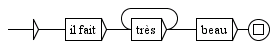
\includegraphics[width=7cm]{resources/img/fig10-1.png}
\caption{Graphe avec un cycle\label{cycle}}
\end{center}
\end{figure}

\end{itemize}







\section{Fst2Txt}\index{Programmes externes!\verb+Fst2Txt+}\index{\verb+Fst2Txt+}
\label{section-Fst2Txt}
\verb+Fst2Txt [OPTIONS] <fst2>+

\bigskip
\noindent Ce programme applique un transducteur à un texte en phase de prétraitement, quand le
texte n’est pas encore découpé en unités lexicales

\bigskip
\noindent \textbf{OPTIONS:}
\begin{itemize}
  \item \verb+-t TXT+/\verb+--text=TXT+: le fichier texte à modifier, avec l’extension \verb+.snt+;
  
  \item \verb+-a ALPH+/\verb+--alphabet=ALPH+: le fichier alphabet de la langue du
  texte;\index{Alphabet}\index{Fichier!alphabet}

  \item \verb+-s+/\verb+--start_on_space+: ce paramètre indique que la recherche va commencer à
  	  n'importe quelle position dans le texte, même avant un espace. Ce paramètre ne devrait
  	  être utilisé que pour effectuer des recherches morphologiques;
  	  
  \item \verb+-x+/\verb+--dont_start_on_space+: interdit au programme de 
  	  reconnaître des séquences commençant par un espace (par défaut);
  
  \item \verb+-c+/\verb+--char_by_char+: ce paramètre facultatif permet d’appliquer le transducteur
  en mode caractère par caractère. Cette option doit être utilisée pour les textes en  langues
  asiatiques comme le Thaï;

  \item \verb+-w+/\verb+--word_by_word+: fonctionne en mode mot par mot (par défaut);
  \item \verb+--input_offsets=XXX+: fichier offset à utiliser.  
\end{itemize}

\bigskip
\noindent \textbf{Options de sorties:}
\begin{itemize}
\item \verb+-M+/\verb+--merge+: ajoute les sorties du transducteur aux séquences reconnues texte
	d'entrée (par défaut);
\item \verb+-R+/\verb+--replace+: remplace les séquences reconnues avec les sorties correspondantes
	du transducteur.
\item \verb+--output_offsets=XXX+: fichier offset à produire	
\end{itemize}

\bigskip
\noindent Ce programme a pour effet de modifier le fichier texte passé en paramètre.







\section{Grf2Fst2}\index{Programmes externes!\verb+Grf2Fst2+}\index{\verb+Grf2Fst2+}
\index{Graphe!compilation}\index{Compilation!d'un graphe}
\verb+Grf2Fst2 [OPTIONS] <grf>+

\bigskip
\noindent \index{Fichier!\verb+.grf+}\index{Fichier!\verb+.fst2+}
Ce programme compile une grammaire en un fichier \verb+.fst2+ (pour plus de détails, voir
section \ref{section-graph-compilation}). Le paramètre \verb+<grf>+ désigne le chemin d’accès
complet au graphe principal de la grammaire, sans omettre l’extension \verb+.grf+.

\bigskip
\noindent \textbf{OPTIONS:}
\begin{itemize}
  \item \verb+-y+/\verb+--loop_check+: active la vérification d'erreurs (
		détection de boucles);
  \item \verb+-n+/\verb+--no_loop_check+: désactive la vérification d'erreurs (par défaut);
  	  \index{Détection d'erreur dans les graphes}\index{Graphe!détection d'erreur}\index{Erreurs dans les graphes}
  \item \verb+-a ALPH+/\verb+--alphabet=ALPH+: spécifie le fichier d’alphabet à utiliser pour faire
  	  le découpage en unités lexicales du contenu des boîtes de la grammaire.

  \item \verb+-c+/\verb+--char_by_char+: le découpage se fait caractère par caractère. Si ni
  	  \verb+-c+ ni \verb+-a+ ne sont utilisés, le découpage s’effectue en prenant des suites de
  	  lettres Unicode.
  \item \verb+-d DIR+/\verb+--pkgdir=DIR+: définit le répertoire de dépôt à utiliser pour compiler
  	  la grammaire (voir section \ref{section-repository}, page \pageref{section-repository}).
  \item \verb+-e+/\verb+--no_empty_graph_warning+: pas d'émission de warning quand les graphes
  	  reconnaissent le mot vide. Cette option est utilisée par \verb+MultiFlex+ pour ne pas
  	  effrayer les utilisateurs par des messages d'erreurs inadéquats lorsqu'ils construisent
  	  une grammaire de flexion qui reconnaît le mot vide.
  \item \verb+-t+/\verb+--tfst_check+: vérifie si le  graphe donné peut être considéré comme un
	automate de phrases ou non;
\item \verb+-s+/\verb+--silent_grf_name+: n'affiche pas le nom des graphes
	(nécessaire pour l'utilisation de fichiers log sur plusieurs systèmes);
\item \verb+-r XXX+/\verb+--named_repositories=XXX+: déclaration de noms de répertoires de dépôt. XXX est formé d'une séquence d'un ou plusieurs X=Y, séparés par `;', où
	X est le nom du répertoire de dépôt désigné par le chemin Y. Vous pouvez utiliser cette option à plusieurs reprises~;
\item \verb+--debug+: compile les graphes en mode  debug;
\item \verb+-v+/\verb+check_variables+: vérifier la validité de sortie afin d'éviter des expressions avec variables malformées.
\end{itemize}

\bigskip
\noindent Le résultat est un fichier portant le même nom que le graphe passé en paramètre, mais
avec l’extension \verb+.fst2+. Ce fichier est sauvegardé dans le même répertoire que \verb+<grf>+.





\section{GrfDiff}
\verb+GrfDiff <grf1> <grf2>: fichier fichiers .grf+  à comparer

\noindent \textbf{OPTIONS:}
\begin{itemize}
\item \verb+--output X+: sauve le résultat éventuel dans X au lieu de l'afficher
\end{itemize}
         
Compare les fichier .grf et affiche leurs différence sur la sortie standard.
Renvoie 0 s'il sont identiques modulo le réordonnancement des boîtes et des transitions, 1 si ils sont différents, 2 en cas d'erreur.
		 
Voici les indications que GrfDiff peut  émettre :
\begin{itemize}
		 
\item \verb+P name+: présentation d'une propriété a changé. name= nom propriété name (SIZE, FONT,
		...)
\item \verb+M a b+:  une boîte est déplacée. a=numéro de boîte dans <grf1>, b=numéro de boîte dans
	<grf2>
\item \verb+C a b+:  le contenu d'une boîte a changé. a=numéro de boîte dans <grf1>, b=numéro de
	boîte dans <grf2>
\item \verb+A x+:    une boîte a été ajoutée. x=numéro de boîte dans <grf2>
\item \verb+R x+:    une boîte a été supprimée. x=numéro de boîte dans <grf1>
\item \verb+T a b x y+: une transition a été ajoutée. a,b=src et dst numéros de boîtes dans <grf1>.
	x,y=src et dst numéros de boîtes dans <grf2>
\item \verb+X a b x y+: transition a été supprimée. a,b=src et dst numéros de boîtes dans <grf1>.
	x,y=src et dst numéros de boîtes dans <grf2>
\end{itemize}
		 
Remarquons que les modifications concernant les transitions liées aux boîtes ajoutées ou supprimées
sont rapportées.





\section{GrfDiff3}
GrfDiff3 <mine> <base> <other>

<mine>: mon fichier .grf
<other>: l'autre fichier .grf qui produit un conflit
<base>: fichier .grf ancêtre commun

\bigskip
\noindent \textbf{OPTIONS:}
\begin{itemize}
\item \verb+--output+ \verb+X+: enregistre le résultat, le cas échéant, dans X et pas sur la sortie
\item \verb+--conflicts+ \verb+X+: enregistre la description des conflits, le cas échéant, dans X
\item \verb+--only-cosmetic+: signale un conflit de tout changement qui n'est pas purement
	cosmétique
\end{itemize}

Essaye de regrouper les <mine> et <other>. En cas de succès, le résultat est imprimé sur la sortie
standard et 0 est renvoyé. En cas de conflits non résolus, 1 est renvoyé et rien n'est imprimé. 2
est renvoyé en cas d'erreur.



\section{ImplodeTfst}
\index{Programmes externes!\verb+ImplodeTfst+}
\index{\verb+ImplodeTfst+} \verb+ImplodeTfst [OPTIONS] <tfst>+

\bigskip
\noindent Ce programme implose l'automate du texte spécifié en fusionnant ensemble les entrées lexicales qui ne diffèrent que par leurs catactéristiques flexionnelles.

\bigskip
\noindent \textbf{OPTIONS:}
\begin{itemize}
\item \verb+-o OUT+/\verb+--output=OUT+: fichier de sortie. Par défaut, l'automate du texte est modifiée.
\end{itemize}






\section{Locate}\index{Programmes externes!\verb+Locate+}\index{\verb+Locate+}
\label{section-Locate}
\verb+Locate [OPTIONS] <fst2>+

\bigskip
\noindent \index{Motif de recherche}
Ce programme applique une grammaire à un texte et construit un fichier d’index des
occurrences trouvées.


\bigskip
\noindent \textbf{OPTIONS:}
\begin{itemize}
\item \verb+-t TXT+/\verb+--text=TXT+: chemin complet du fichier texte, 
  sans omettre l’extension \verb+.snt+;

  \item \verb+-a ALPH+/\verb+--alphabet=ALPH+: chemin d’accès complet au fichier
  	  alphabet;\index{Alphabet}\index{Fichier!alphabet}
  
  \item \verb+-m DICS+/\verb+--morpho=DICS+: ce paramètre optionnel indique
  	  quels dictionnaires morphologiques sont utilisés, s'ils sont exigés par des dictionnaires
  	  \verb+.fst2+
  	  \verb+DICS+ représente une liste de fichiers \verb+.bin+  (avec leurs chemins complets)
  	  séparés par des points-virgules;
  
  \item \verb+-s+/\verb+--start_on_space+: ce paramètre indique que la recherche va commencer à
  	  n'importe quelle position dans le texte, même avant un espace. Ce paramètre ne devrait
  	  être utilisé que pour effectuer des recherches morphologiques;
  
  \item \verb+-x+/\verb+--dont_start_on_space+: interdit au programme de 
  	  reconnaitre des séquences commençant par un espace (par défaut);
	
  \item \verb+-c+/\verb+--char_by_char+: ce paramètre facultatif permet d’appliquer le transducteur
  en mode caractère par caractère. Cette option doit être utilisée pour les textes en  langues
  asiatiques comme le Thaï;
  
  \item \verb+-w+/\verb+--word_by_word+: fonctionne en mode mot par mot (par défaut);
  
\item \verb+-d DIR+/\verb+--sntdir=DIR+: met les fichiers produits dans le répertoire au lieu
	\verb+DIR+ au lieu du répertoire texte. Notez que \verb+DIR+ doit se terminer par un
	séparateur de fichier (\verb+\+ or \verb+/+);
  
  \item \verb+-K+/\verb+--korean+: indique \verb+Locate+ qu'il travaille sur du coréen;

  \item \verb+-u X+/\verb+--arabic_rules=X+: désigne le fichier de configuration des règles
  	  typographiques de l'arabe;

  \item \verb+-g X+/\verb+--negation_operator=X+: spécifie l'opérateur de négation à utiliser dans
  	  les masques lexicaux. Les deux valeurs possibles de \verb+X+ sont \verb+moins+ et
  	  \verb+tilde+ (par défaut).
 Utiliser \verb+moins+ offre une compatibilité descendante avec les versions précédentes de Unitex.
\end{itemize}

\bigskip
\noindent \textbf{Options de limite de recherche:}
\begin{itemize}
\item \verb+-l+/\verb+--all+: recherche toutes les séquences reconnues (par défaut);
\item \verb+-n N+/\verb+--number_of_matches=N+: stoppe après les premiers
  \verb+N+ matches.
\end{itemize}

\bigskip
\noindent \textbf{Options du nombre d'itérations maximum par token:}
\begin{itemize}
\item \verb+-o N+/\verb+--stop_token_count=N+: stoppe après N itérations sur un token;
\item \verb+-o N,M+/\verb+--stop_token_count=N,M+: émet un warning après N itérations sur un token
	et s'arrête après itérations M.
\end{itemize}

\bigskip
\noindent \textbf{Options du mode de reconnaissance:}
\begin{itemize}
  \item \verb+-S+/\verb+--shortest_matches+;
  \item \verb+-L+/\verb+--longest_matches+ (par défaut);
  \item \verb+-A+/\verb+--all_matches+.
\end{itemize}

\bigskip
\noindent \textbf{Options de sortie:}
\begin{itemize}
\item \verb+-I+/\verb+--ignore+: ignore les sorties du transducteur (par défaut);
\item \verb+-M+/\verb+--merge+: ajoute les sorties du transducteur avec les séquences reconnues;
\item \verb+-R+/\verb+--replace+: remplace les séquences reconnues par les sorties correspondantes
	du transducteur;
\item \verb+-p+/\verb+--protect_dic_chars+: quand le mode \verb+-M+ ou \verb+-R+  est utilisé,
	\verb+-p+ protège certains caractères de l'entrée avec un antislash.
	Ceci est utile quand \verb+Locate+ est appelée par \verb+Dico+ afin d'éviter la production
	de mauvaises lignes comme:
  
  %do not remove this line jump
  \verb+3,14,.PI.NUM+
  \item \verb+-v X=Y+/\verb+--variable=X=Y+: définit une variable de sortie nommé \verb+X+ avec un contenu
  	  \verb+Y+. 
  	  Remarquons que Y doit être ASCII.
\end{itemize}

\bigskip
\noindent \textbf{Options de sortie ambiguës:}
\begin{itemize}
  \item \verb+-b+/\verb+--ambiguous_outputs+: permet la production de plusieurs
   matchs avec la même entrée, mais différentes sorties (par défaut);
\item \verb+-z+/\verb+--no_ambiguous_outputs+: interdit les sorties ambiguës. Dans
	le cas de sorties ambiguës, l'une sera arbitrairement choisie, en fonction de l'état interne
	du programme.
\end{itemize}

\bigskip
\noindent \textbf{Options d'erreur sur les variables}

\noindent Ces options n'ont aucun effet si le mode de sortie est réglé avec 
\verb+--ignore+; sinon, elles définissent le comportement du programme  \verb+Locate+
quand une sortie contient une référence à une variable qui n'est pas correctement définie.
\begin{itemize}
\item \verb+-X+/\verb+--exit_on_variable_error+: arrête le programme;
\item \verb+-Y+/\verb+--ignore_variable_errors+: agit comme si la variable avait
   un contenu vide (par défaut);
\item \verb+-Z+/\verb+--backtrack_on_variable_errors+: arrêter d'explorer le chemin courant de la
	grammaire.
\end{itemize}
  
\bigskip
\noindent \textbf{Injection de variables:}
\begin{itemize}
\item \verb+-v X=Y+/\verb+--variable=X=Y+: définit une variable de sortie nommée X avec un
		contenu Y.  
  Notez que Y doit être ASCII.
\end{itemize}

\bigskip
\noindent \index{Fichier!\verb+concord.ind+}\index{Fichier!\verb+concord.n+} Ce
programme enregistre les références des occurrences trouvées dans un fichier appelé
\verb+concord.ind+. Le nombre d'occurrences, le nombre d'unités appartenant à ces
occurrences, ainsi que le pourcentage d'unités reconnues dans le texte sont
enregistrées dans un fichier appelé
\verb+concord.n+. Ces deux fichiers sont stockés dans le répertoire du texte.







\section{LocateTfst}\index{Programmes externes!\verb+LocateTfst+}\index{\verb+LocateTfst+}
\label{section-LocateTfst}
\verb+LocateTfst [OPTIONS] <fst2>+

\bigskip
\noindent \index{Recherche de motifs}
Ce programme applique une grammaire à l'automate du texte, et sauve l'indes des séquences reconnues dans un fichier \verb+concord.ind+, comme le fait \verb+Locate+.

\bigskip
\noindent \textbf{OPTIONS:}
\begin{itemize}
  \item \verb+-t TFST+/\verb+--text=TFST+: chemin complet du fichier texte, 
  sans omettre l’extension;

  \item \verb+-a ALPH+/\verb+--alphabet=ALPH+: chemin d’accès complet au fichier
  	  alphabet;\index{Alphabet}\index{Fichier!alphabet}
  
  \item \verb+-K+/\verb+--korean+: indique à \verb+LocateTfst+ qu'il travaille sur du coréen;

  \item \verb+-g X+/\verb+--negation_operator=X+: spécifie l'opérateur de négation à utiliser dans
  	  les masques lexicaux. Les deux valeurs possibles de \verb+X+ sont \verb+moins+ et \verb+tilde+
  	  (par défaut).
  Utiliser \verb+moins+  offre une compatibilité descendante avec les versions précédentes de
  Unitex.
  
\end{itemize}

\bigskip
\noindent \textbf{Options de limite de recherche:}
\begin{itemize}
  \item \verb+-l+/\verb+--all+: recherche toutes les séquences reconnues (par défaut);
  \item \verb+-n N+/\verb+--number_of_matches=N+: stoppe après les premiers
  \verb+N+ matches.
\end{itemize}

\bigskip
\noindent \textbf{Options du mode de reconnaissance:}
\begin{itemize}
  \item \verb+-S+/\verb+--shortest_matches+;
  \item \verb+-L+/\verb+--longest_matches+ (par défaut);
  \item \verb+-A+/\verb+--all_matches+.
\end{itemize}

\bigskip
\noindent \textbf{Options de sortie:}
\begin{itemize}
  \item \verb+-I+/\verb+--ignore+: ignore les sorties du transducteur (par défaut);
  \item \verb+-M+/\verb+--merge+: ajoute les sorties du transducteur avec les séquences reconnues;
  \item \verb+-R+/\verb+--replace+: remplace les séquences reconnues par les sorties correspondantes
  	  du transducteur;
\end{itemize}

\bigskip
\noindent \textbf{Options de sortie ambiguës:}
\begin{itemize}
  \item \verb+-b+/\verb+--ambiguous_outputs+: permet la production de plusieurs
   matchs avec la même entrée, mais différentes sorties (par défaut);
  \item \verb+-z+/\verb+--no_ambiguous_outputs+: interdit les sorties ambiguës. Dans
	le cas de sorties ambiguës, l'une sera arbitrairement choisie, en fonction de l'état interne
	du programme.
\end{itemize}

\bigskip
\noindent \textbf{Options d'erreur sur les variables}

\noindent Ces options n'ont aucun effet si le mode de sortie est réglé avec
\verb+--ignore+; sinon, elles définissent le comportement du programme \verb+Locate+ 
quand une sortie une référence à une variable qui n'est pas correctement définie.
\begin{itemize}
\item \verb+-X+/\verb+--exit_on_variable_error+: arrête le programme;
\item \verb+-Y+/\verb+--ignore_variable_errors+: agit comme si la variable avait
   un contenu vide (par défaut);
\item \verb+-Z+/\verb+--backtrack_on_variable_errors+:arrêter d'explorer le chemin courant de la
	grammaire.
\end{itemize}
\noindent \textbf{Injection de variables}
\begin{itemize}
\item \verb+-v X=Y+/\verb+--variable=X=Y+: définit une variable de sortie nommée \verb+X+ avec un contenu
  	  \verb+Y+.  
  Notez que Y doit être ASCII.
\end{itemize}
\noindent \textbf{Option d'étiquetage}
\begin{itemize}
\item \verb+--tagging+: indique que la concordance doit être tagguée, et contenir les
  informations supplémentaires sur les états de début et de fin de chaque match.
\end{itemize}
\bigskip
\noindent \index{Fichier!\verb+concord.ind+}\index{Fichier!\verb+concord_tfst.n+}Ce
programme enregistre les références des occurrences trouvées dans un fichier appelé
\verb+concord.ind+. Le nombre d'occurrences, et le nombre de sorties produites sont enregistrées
dans un fichier appelé \verb+concord_tfst.n+. Ces deux fichiers sont stockés dans
le répertoire du texte.







\section{MultiFlex}\index{Programmes externes!\verb+MultiFlex+}\index{\verb+MultiFlex+}
\verb+MultiFlex [OPTIONS] <dela>+

\bigskip
\noindent \index{Dictionnaire!flexion automatique}\index{Flexion automatique}Ce programme effectue
la flexion automatique d'un dictionnaire DELA contenant des formes canoniques 
\ref{section-DELAS-format}) de mots simples ou composés (see chapter \ref{chap-multiflex}).

\bigskip
\noindent \textbf{OPTIONS:}
\begin{itemize}
\item \verb+-o DELAF+/\verb+--output=DELAF+: fichier DELAF de sortie;
  \item \verb+-a ALPH+/\verb+--alphabet=ALPH+: fichier alphabet;
  \item \verb+-d DIR+/\verb+--directory=DIR+: le répertoire contenant les fichiers 
  	  \verb+Morphology+ et \verb+Equivalences+ et des graphes de flexion pour mots
  	  simples ou composés;
  \item \verb+-K+/\verb+--korean+: indique à \verb+MultiFlex+ qu'il travaille sur du coréen;
  \item \verb+-s+/\verb+--only-simple-words+: le programme tiendra compte des mots composés comme
  	  des erreurs;
  \item \verb+-c+/\verb+--only-compound-words+: le programme tiendra compte des mots simples comme
  	  des erreurs;
  \item \verb+-p DIR+/\verb+--pkgdir=DIR+: indique le répertoire des graphes.
  \item \verb+-rXXX+/\verb+--named_repositories=XXX+: déclaration des dépôts nommés. XXX est formée
  	  d'une séquence ou plus X=Y , séparés par ; où X est le nom de dépôt désigné par le chemin
  	  Y. Vous pouvez utiliser cette option à plusieurs reprises;
  
\end{itemize}\index{Hangul}\index{Hangul}

\bigskip
\noindent Remarquons que les transducteurs de flexion \verb+.fst2+ sont automatiquement construits à
partir des fichiers \verb+.grf+ correspondants en cas d'absence ou de fichiers \verb+.grf+ plus
anciens.







\section{Normalize}\index{Programmes externes!\verb+Normalize+}\index{\verb+Normalize+}
\label{section-Normalize}
\index{Texte!normalisation}
\verb+Normalize [OPTIONS] <text>+

\bigskip
\noindent \index{Normalisation!des séparateurs} 
Ce programme effectue une normalisation des séparateurs de texte. Les séparateurs sont l'espace, la
tabulation, et le saut de ligne. Chaque séquence de séparateurs qui contient au moins un saut de
ligne est remplacé par un saut de ligne unique. Toutes les autres séquences de séparateurs sont
remplacées par un seul espace.

\bigskip
\noindent Ce programme vérifie également la syntaxe des étiquettes lexicales présentes dans le
texte. Toute séquence entre accolades doit être soit le délimiteur de phrase \verb+{S}+,
le marqueur \verb+{STOP}+, soit une ligne de DELAF valide (\verb+{aujourd'hui,.ADV}+). 
\index{\verb+{S}+}\index{Délimiteur de phrase}

\bigskip
\noindent \index{Étiquette lexicale} Le paramètre \verb+<text>+ doit représenter le chemin d’accès complet au fichier du texte. Le programme produit une version modifiée du texte qui est sauvé dans
un fichier portant l’extension \verb+.snt+.\index{Fichier!\verb+.snt+}

\bigskip
\noindent \textbf{OPTIONS:}
\begin{itemize}
\item \verb+-n+/\verb+--no_carriage_return+: chaque séquence de séparateurs sera transformée en un
	espace unique;
\item \verb+--input_offsets=XXX+: fichier offset à utiliser.
\item \verb+--output_offsets=XXX+: fichier offset à  produire
\item \verb+-r XXX+/\verb+--replacement_rules=XXX+: indique la règle de normalisation à utiliser.
	Voir section \ref{section-normalization-file} Pour plus de détails sur le format de
	ce fichier. Par défaut, le programme ne remplace que \verb+{+ and \verb+}+ par \verb+[+ et
	\verb+]+.
\item \verb+--no_separator_normalization+: n'applique que des règles de remplacement  spécifiées par
	-r
\end{itemize}

\bigskip
\noindent ATTENTION: si vous spécifiez un fichier de règles de normalisation, ces règles seront
appliquées avant toute autre chose. Donc, il faut être très prudent si vous manipulez les
séparateurs dans ces règles.






\section{PolyLex}\index{Programmes externes!\verb+PolyLex+}\index{\verb+PolyLex+}
\verb+PolyLex [OPTIONS] <list>+
\index{Norvégien!mots composés libres}
\index{Allemand!mots composés libres}
\index{Néerlandais!mots composés libres}
\index{Russe!mots composés libres}
\index{Analyse des mots composés libres!langues germaniques}
\index{Mots!composés libres!langues germaniques}
\index{Analyse des mots composés libres!russe}
\index{Mots!composés libres!russe}

\bigskip
\noindent Ce programme prend en paramètre un fichier de mots inconnus \verb+<list>+ et essaye d’analyser chacun d’eux comme un mot composé obtenu par soudure de mots simples. Les mots
qui ont au moins une analyse sont retirés du fichier de mots inconnus et les lignes de dictionnaire
correspondant aux analyses sont ajoutées au fichier \verb+OUT+.

\bigskip
\noindent \textbf{OPTIONS:}
\begin{itemize}
  \item \verb+-a ALPH+/\verb+--alphabet=ALPH+: le fichier alphabet à utiliser;

  \item \verb+-d BIN+/\verb+--dictionary=BIN+: le dictionnaire .bin à utiliser;

  \item \verb+-o OUT+/\verb+--output=OUT+: désigne le fichier dans lequel les
  lignes de dictionnaire produites doivent être enregistrées, si ce fichier existe déjà,
  les lignes sont ajoutées à la fin du fichier;

  \item \verb+-i INFO+/\verb+--info=INFO+: désigne un fichier texte dans lequel
   les informations relatives à l'analyse a été réalisée.
\end{itemize}

\bigskip
\noindent \textbf{Options de langue:}
\begin{itemize}
  \item \verb+-D+/\verb+--dutch+
  \item \verb+-G+/\verb+--german+
  \item \verb+-N+/\verb+--norwegian+
  \item \verb+-R+/\verb+--russian+
\end{itemize}  

\bigskip
\noindent NOTE: pour les mots hollandais ou norvégiens, le programme tente de lire un fichier texte
contenant une liste de mots interdits. Ce fichier est supposé s'appeler
\verb+ForbiddenWords.txt+ (voir section \ref{section-forbidden-words}) et être stocké
dans le même répertoire que \verb+BIN+.



\section{RebuildTfst}
\index{Programmes externes!\verb+RebuildTfst+}\index{\verb+RebuildTfst+}
\verb+RebuildTfst <tfst>+

\bigskip
\noindent \index{Texte!automate du}\index{Reconstruction de l'automate du texte}Ce programme reconstruit l'automate du texte \verb+<tfst>+ en tenant compte des modifications manuelles. Si le programme trouve un fichier \verb+sentenceN.grf+ dans le même répertoire que \verb+<tfst>+, il remplace l'automate de la phrase \verb+N+ par celle représentée par \verb+sentenceN.grf+. L'automate du texte donné entrée est modifié.






\section{Reconstrucao}\index{Programmes externes!\verb+Reconstrucao+}\index{\verb+Reconstrucao+}
\index{Compression des dictionnaires}\index{Dictionnaire!compression}
\index{Clitiques!normalisation}\index{Normalisation!des clitiques en portugais}
\index{Portugais!normalisation des clitiques}
\verb+Reconstrucao [OPTIONS] <index>+

\bigskip
\noindent Le programme génère une grammaire de normalisation destinée à être appliquée
avant la construction d'un automate pour un texte en langue portugaise. Le fichier \verb+<index>+ 
représente une concordance qui doit être produite en mode MERGE to
the considered text a grammar that extracts all forms to be normalized. Cette
grammaire est nommée \verb+V-Pro-Suf+, et est stockée dans le répertoire
\verb+/Portuguese/Graphs/Normalization+.

\bigskip
\noindent \textbf{OPTIONS:}
\begin{itemize}
  \item \verb+-a ALPH+/\verb+--alphabet=ALPH+: le fichier alphabet à utiliser;

  \item \verb+-r ROOT+/\verb+--root=ROOT+: le dictionnaire inversé \verb+.bin+
  	  à utiliser pour retrouver les formes au futur et au conditionnel à partir des formes
  	  canoniques. Il a été obtenu en compressant le dictionnaire des verbes au futur
  	  et au conditionnel avec le paramètre \verb+--flip+ (voir section \ref{section-compress});
  
  \item \verb+-d BIN+/\verb+--dictionary=BIN+: le dictionnaire \verb+.bin+ à utiliser;
  
  \item \verb+-p PRO+/\verb+--pronoun_rules=PRO+: la grammaire \verb+.fst2+ de réécriture des pronoms;

  \item \verb+-n PRO+/\verb+--nasal_pronoun_rules=PRO+: la grammaire \verb+.fst2+ de réécriture des pronoms nasaux;

  \item \verb+-o OUT+/\verb+--output=OUT+: le nom du graphe \verb+.grf+ à générer
\end{itemize}







\section{Reg2Grf}\index{Programmes externes!\verb+Reg2Grf+}\index{\verb+Reg2Grf+}
\verb+Reg2Grf <txt>+

\bigskip
\noindent \index{Expression régulière} \index{Expression rationnelle}
\index{Fichier!\verb+.grf+}\index{Fichier!\verb+regexp.grf+}Ce programme construit un fichier
\verb+.grf+ correspondant à l’expression rationnelle contenue dans le fichier \verb+<txt>+.
Le paramètre \verb+<txt>+ doit représenter le chemin d’accès complet au fichier contenant
l’expression rationnelle. Ce fichier doit être un fichier texte Unicode. Le programme prend en
compte tous les caractères jusqu’au premier retour à ligne. Le fichier résultat se nomme
\verb+regexp.grf+ et est sauvegardé dans le même répertoire que \verb+<txt>+.





\section{Seq2Grf}\index{Programmes externes!\verb+Seq2Grf+}
\index{\verb+Seq2Grf+}
\label{Seq2Grf}
\verb+Seq2Grf [OPTIONS] <snt>+

\index{Tri}
\bigskip
\noindent ce programme construit un fichier \verb+.grf+ 
qui correspond aux séquences contenues dans le fichier \verb+<snt>+.

\bigskip
\noindent \textbf{OPTIONS:}

\begin{itemize}
  \item \verb+-a ALPH+/\verb+--alphabet=ALPH+: le fichier alphabet à utiliser;
  \item \verb+-o XXX+/\verb+--output=XXX+: le fichier graphe de sortie;
  \item \verb+-s+/\verb+--only-stop+: ne considérer que les séquences séparées par \verb+{STOP}+;
  \item \verb+-b+/\verb+--beautify+: appliquer au graphe l'algorithme beautify;
  \item \verb+-n+/\verb+--no_beautify+: ne pas appliquer au graphe l'algorithme beautify; (par défaut);
  \item \verb+--case-sensitive+: respect de la casse (par défaut);
  \item \verb+--case-insensitive+: non respect de la casse;
  \item \verb+-w x+: nombre de jokers;
  \item \verb+-i x+: nombre d'insertions;
  \item \verb+-r x+: nombre de remplacement;
  \item \verb+-d x+: nombre de délitions;
\end{itemize}

\bigskip
\noindent Construire l'automate des séquences : un unique automate qui reconnaît toutes les séquences du SNT. Les  séquences doivent être  délimitées par l'étiquette \verb+{STOP}+;. Le fichier
\verb+.grf+ produit est stocké dans le répertoire Graphs de l'utilisateur. Les autres fichiers,
nommés \verb+text.tfst+, \verb+text.tind+ se trouvent dans le répertoire text.

\section{SortTxt}\index{Programmes externes!\verb+SortTxt+}\index{\verb+SortTxt+}

\verb+SortTxt [OPTIONS] <txt>+

\index{Tri}
\bigskip
\noindent Ce programme effectue un tri lexicographique des lignes du fichier
\verb+<txt>+. \verb+<txt>+ doit représenter le chemin d’accès complet au fichier à trier.


\bigskip
\noindent \textbf{OPTIONS:}
\begin{itemize}
\item \verb+-n+/\verb+--no_duplicates+: supprime les doublons (par défaut);

\item \verb+-d+/\verb+--duplicates+: conserve les doublons;

\item \verb+-r+/\verb+--reverse+: trie en ordre décroissant;

\item \verb+-o XXX+/\verb+--sort_order=XXX+: trie en utilisant l'ordre alphabétique défini par le
fichier \verb+XXX+. Si ce paramètre est abscent, le tri est effectué selon l'ordre des caractères
Unicode;

\item \verb+-l XXX+/\verb+--line_info=XXX+: sauvegarde le nombre de lignes du fichier résultat dans le fichier \verb+XXX+;
  
\item \verb+-t+/\verb+--thai+: option à utiliser pour trier un texte Thai.
\item \verb+-f+/\verb+--factorize_inflectional_codes+: transforme les deux entrées XXX,YYY.ZZZ:A et XXX,YYY.ZZZ:B en l'entrée unique  XXX,YYY.ZZZ:A:B
\end{itemize}

\bigskip
\noindent L’opération de tri modifie le fichier texte. Par défaut, le tri est effectué dans l’ordre
des caractères en Unicode, en supprimant les doublons.









\section{Stats}\index{Programmes externes!\verb+Stats+}\index{\verb+Stats+}

\verb+Stats [OPTIONS] <ind>+

\index{Statistiques}
\bigskip
\noindent Ce programme calcule des statistiques à partir du fichier d'index de concordances \verb+<ind>+.

\bigskip
\noindent \textbf{OPTIONS:}
\begin{itemize}
\item \verb+-m MODE+/\verb+--mode=MODE+: spécifie la sortie à produire:
  \begin{itemize}
  \item \verb+0+ = séquence reconnue avec contexte gauche et droit + nombre d'occurrences;
  \item \verb+1+ = cooccurrences + nombre d'occurrences;
      \item \verb+2+ = cooccurrences + nombre d'occurrences + z-score.
  \end{itemize}

  \item \verb+-a ALPH+/\verb+--alphabet=ALPH+: fichier alphabet à utiliser;

  \item \verb+-o OUT+/\verb+--output=OUT+: fichier de sortie;

  \item \verb+-l N+/\verb+--left=N+: longueur du contexte gauche en tokens;
   
  \item \verb+-r N+/\verb+--right=N+: longueur du contexte droit en tokens;
  
  \item \verb+-c N+/\verb+--case=N+: traitement de la casse: \verb+0+ = non respect de la casse,
  	  \verb+1+ = respect de la casse (par défaut).
\end{itemize}







\section{Table2Grf}\index{Programmes externes!\verb+Table2Grf+}\index{\verb+Table2Grf+}
\verb+Table2Grf [OPTIONS] <table>+

\bigskip
\noindent \index{Lexique-grammaire!table}\index{Graphe!principal}
Ce programme génère automatiquemient des graphes à partir de la table de lexique-
grammaire \verb+<table>+ et d'un graphe patron

\bigskip
\noindent \textbf{OPTIONS:}
\begin{itemize}
\item \verb+-r GRF+/\verb+--reference_graph=GRF+: nom du graphe patron;
  
\item \verb+-o OUT+/\verb+--output=OUT+: nom du graphe résultant principal;
  
  \item \verb+-s XXX+/\verb+--subgraph_pattern=XXX+: si ce paramètre optionnel est spécifié, tous
  	  les sous-graphes produits seront nommés en fonction de ce motif. Afin d'avoir des noms non
  	  ambigus, nous vous recommandons d'inclure \verb+@%+ dans le paramètre
   (rappelons que \verb+@%+ sera remplacé par le numéro de ligne de l'entrée dans la table).
   Par exemple, si vous définissez le paramètre par le motif '\verb+subgraph-@%.grf+', 
   les noms de sous-graphe seront de la forme '\verb+subgraph-0013.grf+'. Par défaut,
   les noms de sous-graphe ressemblent à '\verb+result_0013.grf+', où '\verb+result.grf+' est le
   graphe résultant principal.
\end{itemize}




\section{Tagger}\index{Programmes externes!\verb+Tagger+}\index{\verb+Tagger+}
\verb+Tagger [OPTIONS] <tfst>+
\label{section-Tagger}

\bigskip
\noindent L'entrée de ce programme est l'automate du texte spécifié dans \verb+.tfst+. Le programme
applique l'algorithme de Viterbi et produit un automate linéaire. L'automate est élagué de façon
probabiliste selon un modèle de Markov caché de second ordre. Si fichier tagger indiqué
contient des tuples de type "cat" , le tagger élague les transitions sur la base des codes grammaticaux, syntaxiques
et sémantiques (par exemple, \verb$that.DET+Ddem$ versus 
	\verb$that.PRO+Pdem$). Par contre si le fichier contient des tuples de type "morph", le tagger élague les transitions
sur la base des codes grammaticaux, syntaxiques, sémantiques et flexionnels (\verb$the.DET+Ddef:s$ versus \verb$the.DET+Ddef:p$). Dans le cas où,
l'automate doit être développé avant d'applique le processus d'étiquetage un fichier tagset doit re indiqué avec l'option \verb+-t+ ci-dessous.

\bigskip
\noindent \textbf{OPTIONS:}
\begin{itemize}
\item \verb+-a ALPH+/\verb+--alphabet=ALPH+: fichier alphabet.
\item \verb+-o OUT+/\verb+--output=OUT+: automate du texte en sortie.
  \item \verb+-t TAGSET+/\verb+--tagset=TAGSET+: nom du fichier tagset.
  \item \verb+-d DATA+/\verb+--data=DATA+: un fichier de donné tagger .bin  qui contient le nombre d'occurences d' 
  	  unigramme, de bigrammes et de  trigrammes afin de calculer des probabilités. ce fichier est fournit avec 
  	  le programme \verb+TrainingTagger+ (voir section \ref{section-training-dict}).
\end{itemize}





\section{TagsetNormTfst}
\index{Programmes externes!\verb+TagsetNormTfst+}
\index{\verb+TagsetNormTfst+} \verb+TagsetNormTfst [OPTIONS] <tfst>+

\bigskip
\noindent Ce programme normalise l’automate de texte \verb+.tfst+ selon
un fichier de jeu d'étiquettes, en supprimmant les codes dictionnaire non déclarés
et les entrées lexicales incohérentes. Les caractéristiques flexionnelles ne pas sont factorisées
afin que \verb+{rouge,.A:fs:ms}+ soit divisé en deux étiquettes \verb+{rouge,.A:fs}+ 
et \verb+{rouge,.A:ms}+.

\bigskip
\noindent \textbf{OPTIONS:}
\begin{itemize}
\item \verb+-o OUT+/\verb+--output=OUT+: automate de texte résultant. Par défaut, l'automate du texte donné en entrée est modifié;
\item \verb+-t TAGSET+/\verb+--tagset=TAGSET+: nom du fichier de description du jeu d'étiquettes
\end{itemize}







\section{TEI2Txt}\index{Programmes externes!\verb+TEI2Txt+} 
\index{\verb+TEI2Txt+}
\verb+TEI2Txt [OPTIONS] <xml>+

\bigskip
\noindent Produit un fichier de texte brut à partir du fichier TEI \verb+<xml>+.

\bigskip
\noindent \textbf{OPTIONS:}
\begin{itemize}
  \item \verb+-o TXT+/\verb+--output=TXT+: nom du fichier de texte de sortie.
  	  Par défaut, le fichier de sortie porte le même nom que celui d'entrée, 
  	  remplaçant \verb+.xml+ by \verb+.txt+.
\end{itemize}







\section{Tfst2Grf}
\index{Programmes externes!\verb+Tfst2Grf+}\index{\verb+Tfst2Grf+}
\index{Automate!du texte}\index{Texte!automate du}
\verb+Tfst2Grf [OPTIONS] <tfst>+

\bigskip
\noindent Ce programme extrait un automate de phrase en format \verb+.grf+ format à partir d'un automate du texte donné.

\bigskip
\noindent \textbf{OPTIONS:}
\begin{itemize}
\item \verb+-s N+/\verb+--sentence=N+: le nombre de phrases à extraire;
  
\item \verb+-o XXX+/\verb+--output=XXX+: motif utilisé pour nommer le fichier de sortie
	\verb+XXX.grf+, \verb+XXX.txt+ et \verb+XXX.tok+ (defaut=\verb+cursentence+);
 
\item \verb+-f FONT+/\verb+--font=FONT+: définit la police à utiliser en sortie \verb+.grf+
   
%DO NOT REMOVE THIS LINE JUMP
  (default=\verb+Times new Roman+);
\item \verb+-z N+/\verb+--fontsize=N+: définit la taille de police (defaut=10).
\end{itemize}

\bigskip
\noindent Le programme produit les fichiers suivants et les enregistre dans le
répertoire du texte:

\begin{itemize}
\item \verb+cursentence.grf+: graphe représentant l'automate de la phrase; \index{Fichier!\verb+cursentence.grf+}

\item \verb+cursentence.txt+: fichier texte contenant la phrase;
\index{Fichier!\verb+cursentence.txt+}

\item \verb+cursentence.tok+: fichier texte contenant le nombre de token qui compose la phrase;
\index{Fichier!\verb+cursentence.tok+}
\end{itemize}







\section{Tfst2Unambig}\index{Programmes externes!\verb+Tfst2Unambig+}\index{\verb+Tfst2Unambig+}
\index{Texte!automate du!conversion en texte linéaire}
\verb+Tfst2Unambig [OPTIONS] <tfst>+

\bigskip
\noindent Ce programme prend un automate de texte \verb$.tfst$ et produit le fichier texte équivalent si celui-ci est linéaire (i.e. sans ambiguïté). Voir section \ref{section-linear-text}, page \pageref{section-linear-text}.

\bigskip
\noindent \textbf{OPTIONS:}
\begin{itemize}
\item \verb+-o TXT+/\verb+--out=TXT+: fichier de sortie.
\end{itemize}







\section{Tokenize}\index{Programmes externes!\verb+Tokenize+}\index{\verb+Tokenize+}
\label{section-Tokenize}
\index{Texte!découpage en unités lexicales}
\verb+Tokenize [OPTIONS] <txt>+

\index{Unité lexicale}
\index{Fichier!\verb+.snt+}\index{Alphabet}\index{Fichier!alphabet} 
\bigskip
\noindent Ce programme découpe le texte en unités lexicales.
\verb+<txt>+ le chemin d’accès complet au fichier texte, sans omettre l’extension \verb+.snt+ 
extension.

\bigskip
\noindent \textbf{OPTIONS:}
\begin{itemize}
  \item \verb+-a ALPH+/\verb+--alphabet=ALPH+: alphabet file;
  
  \item \verb+-c+/\verb+--char_by_char+: indique que le  programme est appliqué caractère
  	  par caractère à l'exception du délimiteur de phrase \verb+{S}+,
  	  du marqueur \verb+{STOP}+ et d'étiquettes lexicales comme \verb+{today,.ADV}+ qui sont considérées comme des unités simples;

 \item \verb+-w+/\verb+--word_by_word+: Avec cette option, le programme 
 	 considère qu'une unité est soit une séquence de lettres (ces lettres sont définies dans le fichier \verb+alphabet+), ou un caractère qui n'est pas une lettre, ou le délimiteur de phrase \verb+{S}+\index{\verb+{S}+}, ou une étiquette lexicale comme
 	 \verb+{aujourd'hui,.ADV}+. \index{Délimiteur de phrase}
   \index{Étiquette lexicale} C'est le mode par défaut.

\item \verb+-t TOKENS+/\verb+--tokens=TOKENS+: désigne un fichier a \verb+tokens.txt+
 à charger et à modifier, au lieu d'en créer un nouveau à partir de zéro.
\end{itemize}
\bigskip
\noindent \textbf{Options d'offsets:}
\begin{itemize}
\item \verb+input_offsets+: fichier offsets d'entrée;
\item \verb+output_offsets+: fichier offsets à  produire;
\end{itemize}


\index{Fichier!\verb+tokens.txt+}\index{Fichier!\verb+text.cod+}
\bigskip
\noindent Le programme code chaque unité par un entier. La liste des unités est sauvegardée dans
un fichier texte nommé \verb+tokens.txt+. La suite des codes représentant les unités permet alors
de coder le texte. Cette suite est sauvegardée dans un fichier binaire nommé \verb+text.cod+.  
Le programme produit également les fichiers suivants :


\begin{itemize}
  \item \verb+tok_by_freq.txt+: fichier texte contenant la liste des unités triées par ordre de
  	  fréquence ;
  \item \verb+tok_by_alph.txt+: fichier texte contenant la liste des unités triées par ordre
  	  alphabétique ;

  \item \verb+stats.n+: fichier texte contenant des informations sur le nombre de séparateurs de
phrases, le nombre d’unités, le nombre de mots simples et le nombre de chiffres ;


  \item \verb+enter.pos+: fichier binaire contenant la liste des positions des retours à la ligne
  dans le texte. La représentation codée du texte ne contient pas de retours à la ligne, mais des
  espaces. Comme un retour à la ligne compte pour 2 caractères et l’espace pour un seul, il faut
  savoir où se trouvent les retours à la ligne dans le texte si l’on veut synchroniser les positions
  des occurrences calculées par le programme \verb+Locate+ avec le fichier texte. Le fichier \verb+enter.pos+ est utilisé à cette fin par le programme \verb+Concord+
  C’est grâce à cela que lorsque l’on clique sur une occurrence dans une concordance, celle-ci est
  correctement sélectionnée dans le texte.

\end{itemize}
\index{Fichier!\verb+tok_by_freq.txt+}\index{Fichier!\verb+tok_by_alph.txt+}
\index{Fichier!\verb+stats.n+}\index{Fichier!\verb+enter.pos+}

\bigskip
\noindent Tous les fichiers produits sont sauvegardés dans le répertoire du texte.






\section{TrainingTagger}\index{Programmes externes!\verb+TrainingTagger+}\index{\verb+TrainingTagger+}
\verb+TrainingTagger [OPTIONS] <txt>+
\label{section-TrainingTagger}

\bigskip
\noindent \index{Lexique-grammaire!table}\index{Graphe!principal}Ce programme génère automatiquement deux
fichiers de données Tagger à partir d'un corpus étiqueté. Ils sont utilisés par le programme
\verb+Tagger+ afin de calculer les probabilités et linéariser l'automate texte. Le fichier corpus
étiqueté doit suivre le format décrit à la section \ref{section-corpus-file}. Ces fichiers
contiennent des tuples (unigrammes, bigrammes et trigrammes), formées par des balises et des mots.
Dans le premier fichier de données, les étiquettes sont de type "cat" (i.e. des codes grammaticaux,
	syntaxiques et sémantiques). 
Dans le second fichier de données, les étiquettes sont de type "morph" (i.e. des codes
	grammaticaux, syntaxiques, sémantiques et flexionnels). 

\bigskip
\noindent \textbf{OPTIONS:}
\begin{itemize}
\item \verb+-a/--all+: indique que le programme doit produire tous les fichiers de données (par
		défaut);
\item \verb+-c/--cat+: indique que le programme ne doit produire que les fichiers de données avec
	"cat";
  \item \verb+-m/--morph+: indique que le programme ne doit produire que les fichiers de données
  	  avec "morph";
  \item \verb+-n/--no_binaries+: indique que le programme ne doit pas compresser les fichiers de
  	  données en fichiers \verb+.bin+, seulement dans ce cas les fichiers de données \verb+.dic+ sont genérés;
  \item \verb+-b/--binaries+: indique que le programme doit compresser les fichiers de données en
  	  fichiers \verb+.bin+ files (par défaut);
  \item \verb+-o XXX/--output=XXX+: motif utilisé pour nommer les fichiers de sortie du taggueur
  	  \verb+XXX_data_cat.bin+; et \verb+XXX_data_morph.bin+ (par défaut: nom de fichier sans
  	  	  extension corpus de textes);
  \item \verb+-s/--semitic+: indique que l'algoritme de compression sémitique doit être utilisé;
\end{itemize}

\bigskip

\section{Txt2Tfst}\index{Programmes externes!\verb+Txt2Tfst+}\index{\verb+Txt2Tfst+} \verb+Txt2Tfst [OPTIONS] <txt>+
\index{Automate!du texte}\index{Texte!automate du}\index{Fichier!\verb+.snt+}
\index{Fichier!alphabet}\index{Alphabet}
\bigskip
\noindent Ce programme construit l’automate du texte. Le paramètre \verb+<txt>+ doit représenter le
chemin d’accès complet au fichier texte, sans omettre l’extension \verb+.snt+


\bigskip
\noindent \textbf{OPTIONS:}
\begin{itemize}
  \item \verb+-a ALPH+/\verb+--alphabet=ALPH+: fichier alphabet;
  
  \item \verb+-c+/\verb+--clean+: indique que la règle de conservation des meilleurs chemins (voir
  		  section \ref{section-keeping-best-paths}) doit être utilisée \index{Conservation des meilleurs chemins};
  
  \item \verb+-n XXX+/\verb+--normalization_grammar=XXX+: nom de la grammaire de normalisation
  	  qui doit être appliquée à l'automate de texte; \index{Normalisation!de formes ambiguës}
  	  \index{Normalisation!de l'automate du texte}
  \item \verb+-t TAGSET+/\verb+--tagset=TAGSET+: fichier de jeu d'étiquete Elag pour la
  	  normalisation des entrées du dictionnaire;
  \item \verb+-K+/\verb+--korean+: indique à \verb+Txt2Tfst+ qu'il traite du coréen.

\end{itemize}

\bigskip
\noindent Si le texte a été découpé en phrases, le programme construit un automate pour chaque
phrase. Si ce n’est pas le cas, le programme découpe arbitrairement le texte en séquences de
2000 unités lexicales et construit un automate pour chacune de ces séquences.
\index{Unité lexicale}

\index{Fichier!\verb+text.tfst+}\index{Fichier!\verb+text.tind+}
\bigskip
\noindent Le résultat est un fichier nommé \verb+text.tfst+ qui est sauvegardé dans le répertoire du
texte. Un autre fichier \verb+text.tind+ est aussi produit.

\bigskip
\noindent NOTE: Ce programme essaye également d'utiliser le fichier \verb+tags.ind+ s'il existe
(voir section \ref{section-tags-ind}).







\section{Uncompress}\index{Programmes externes!\verb+Uncompress+}\index{\verb+Uncompress+}
\label{section-Uncompress}
\verb+Uncompress [OPTIONS] <bin>+

\bigskip
\noindent Ce programme décompresse un dictionnaire \verb+.bin+ en un fichier texte
\verb+.dic+.

\bigskip
\noindent \textbf{OPTIONS:}
\begin{itemize}
\item \verb+-o OUT+/\verb+--output=OUT+: nom du fichier de sortie optionnel (par défaut:
  \verb+file.bin+ > \verb+file.dic+).
\end{itemize}








\section{Untokenize}\index{Programmes externes!\verb+Untokenize+}\index{\verb+Untokenize+}
\label{section-Untokenize}
\verb+Untokenize [OPTIONS] <txt>+

\bigskip
\noindent Untokenize et reconstruit le texte orgininal. La liste des token est stockée dans le
fichier \verb+tokens.txt+ et le texte codé dans \verb+text.cod+.
Le fichier \verb+enter.pos+ contient la position en tokens de tous les retours à la ligne
Ces fichiers se trouvent dans le répertoire XXX\_snt où XXX est sans son extension <txt>.

\bigskip
\noindent \textbf{OPTIONS:}
\begin{itemize}

\item \verb+-d X+/\verb+--sntdir=X+: utilise le répertoire X au lieu du répertoire texte; remarquez que X doit se terminer par un antislash
\item \verb+-n N+/\verb+--number_token=N+: ajoute le numéro de token chaque N token;
\item \verb+-r N+/\verb+--range=N+: émet seulement les tokens du numéro N à la fin;
  \item \verb+-r N,M+/\verb+--range=N,M+: émet seulement les tokens du numéro N à M.
\end{itemize}








\section{UnitexTool}
\index{Programmes externes!\verb+UnitexTool+}\index{\verb+UnitexTool+}\index{Script de programmes Unitex}
\label{section-UnitexTool}
\verb+UnitexTool <utilities>+

\bigskip
\noindent Ce programme est un programme qui vous permet d'exécuter tous les programmes externes
d'Unitex
Avec lui, vous pouvez enchaîner les commandes afin qu'elles soit exécutées dans un même processus,
afin d'accélérer le traitement. Cela se fait en invoquant des commandes imbriquées entre parenthèses
comme ceci:

\bigskip
\begin{verbatim}
UnitexTool { SelectOutput [OPTIONS] } 
                { cmd #1+args } 
                { cmd #2+args }
                etc.
\end{verbatim}

\bigskip
\noindent Par exemple, si vous souhaitez faire un locate et construire la  concordance, vous pouvez
utiliser la commande suivante:

\bigskip
\begin{verbatim}
UnitexTool { Locate "-tD:\My Unitex\English\Corpus\ivanhoe.snt" 
"D:\My Unitex\English\regexp.fst2"
"-aD:\My Unitex\English\Alphabet.txt" -L -I -n200 
"--morpho=D:\Unitex2.0\English\Dela\dela-en-public.bin" -b -Y }
{ Concord "D:\My Unitex\English\Corpus\ivanhoe_snt\concord.ind" 
"-fCourier new" -s12 -l40 -r55 --CL --html 
"-aD:\My Unitex\English\Alphabet_sort.txt" }
\end{verbatim}
 
\bigskip
\noindent \textbf{OPTIONS}:
\begin{itemize}
\item \verb+-o [on/off]+/\verb+--output=[on/off]+: activer (on) ou désactiver (off) la sortie standard
\item \verb+-e [on/off]+/\verb+--error=[on/off]+: activer (on) ou désactiver (off) la sortie erreur standard
\end{itemize} 
 
\noindent Par exemple:
\begin{verbatim}
UnitexTool { SelectOutput -o off -e off } { Normalize
Unitex\English\Corpus\ivanhoe.txt }
\end{verbatim}






\section{UnitexToolLogger}\index{Programmes externes!\verb+UnitexToolLogger+}\index{\verb+UnitexToolLogger+}\index{Log programmes Unitex}
\label{section-UnitexToolLogger}
\verb+UnitexToolLogger <utilities>+

\bigskip
\noindent Ce programme est un surensemble de UnitexTool. Il permet d'exécuter à nouveau un
fichier de log .ulp.
Il peut également enregistrer une session d'UnitexTool en cours d'exécution et créer un fichier de
log .ulp.
Si UnitexToolLogger est utilisé comme UnitexTool (avec uniquement les paramètres contenant des lignes de
	commande pour des programmes Unitex externes), et qu'un fichier contenant un chemin et nommé
unitex\_logging\_parameters\_count.txt est présent dans le répertoire courant, alors
un fichier de log .ulp pour la session en cours sera créé.
Le fichier .ulp est un fichier zip comprimé (compatible avec unzip), qui peut être utile pour le débogage.

\bigskip
\verb+UnitexToolLogger RunLog [OPTIONS] <ulp>+

\bigskip
\noindent \textbf{OPTIONS after RunLog:}
\begin{itemize}
  \item \verb+-m+/\verb+--quiet+: n'émet pas de messages lors de l'exécution;
  \item \verb+-v+/\verb+--verbose+: émet des messages lors de l'exécution;
  
  \item \verb+-d DIR+/\verb+--rundir=DIR+: chemin où le fichier log est exécuté;
  \item \verb+-r newfile.ulp+/\verb+--result=newfile.ulp+: nom du fichier ulp résultat créé;

  \item \verb+-c+/\verb+--clean+: supprime le fichier de travail après l'exécution;
  \item \verb+-k+/\verb+--keep+: conserve le fichier de travail après l'exécution;

  \item \verb+-s file.txt+/\verb+--summary=file.txt+: fichier ** avec comparaison de log
  \item \verb+-e file.txt+/\verb+--summary-error=file.txt+: fichier de synthèse avec comparaison des
  	  erreurs;

  \item \verb+-b+/\verb+--no-benchmark+: ne pas enregistrer le temps d'exécution dans les fichiers
  	  log;

  \item \verb+-n+/\verb+--cleanlog+: supprime le résultat ulp après exécution;
  \item \verb+-l+/\verb+--keeplog+: garde le résultat ulp après exécution;

  \item \verb+-o NameTool+/\verb+--tool=NameTool+: lance seulement les log pour \verb+NameTool+;
  \item \verb+-i N+/\verb+--increment=N+: incrémenter le nom de fichier <ulp> de  0 à N;
  \item \verb+-t N+/\verb+--thread=N+: créer N thread;
  \item \verb+-a N+/\verb+--random=N+: choisir N fois un fichier log aléatoire dans la liste (dans chaque thread);
  \item \verb+-f N+/\verb+--break-after=N+: l'utilisateur annule après N exécutions (avec seulement un seul thread);

  \item \verb+-u PATH+/\verb+--unfound-location=PATH+: prend le dictionnaire et le FST2 à partir de  PATH s'il est absent du fichier log;
\end{itemize}


Une autre utilisation UnitexToolLogger  est d'utiliser l'option MzRepairUlp pour réparer un fichier ulp abîmé (souvent, un log de crash):

\bigskip
\verb+UnitexToolLogger MzRepairUlp [OPTIONS] <ulpfile>+

\bigskip
\noindent \textbf{OPTIONS après MzRepairUlp:}
\begin{itemize}
\item \verb+-t X+/\verb+--temp=X+: utilise  X comme nom de fichier temporaire (<ulpfile>.build par défaut);
\item \verb+-o X+/\verb+--output=X+: utilise X comme nom de fichier .ulp  (<ulpfile>.repair par défaut);
  \item \verb+-m+/\verb+--quiet+: n'émet pas de message lors de l'exécution;;
  \item \verb+-v+/\verb+--verbose+: émet un message lors de l'exécution;
\end{itemize}


Une autre utilisation de UnitexToolLogger est d'utiliser l'option CreateLog option (avec des accolades) pour créer un fichier log d'exécutions de programme Unitex, comme:

\bigskip
\noindent \verb$UnitexToolLogger { CreateLog [OPTIONS] } cmd args$

\bigskip
\noindent \verb$UnitexToolLogger { CreateLog [OPTIONS] } { cmd #1+args } { cmd #2+args } etc.$

\noindent Par exemple,
\begin{verbatim}
UnitexToolLogger { CreateLog --log_file=my_run_normalize.ulp }
             Normalize "C:\My Unitex\French\Corpus\80jours.txt"
\end{verbatim}

\bigskip
\begin{verbatim}
UnitexToolLogger { CreateLog --directory=c:\logs }
                  { Compress c:\dela\mydela.dic }
                  { CheckDic --delaf c:\dela\mydela.inf }
\end{verbatim}

\bigskip
\noindent \textbf{OPTIONS après CreateLog:}
\begin{itemize}
\item \verb+-g+/\verb+--no_create_log+: ne pas créer de fichier log. Incompatible avec toutes les autres options;

\item \verb+-p XXX+/\verb+--param_file=XXX+: charge un fichier de paramètres comme unitex\_logging\_parameters.txt. Incompatible avec toutes les autres options;

\item \verb+-d XXX/--directory=XXX+: Emplacement du répertoire où le fichier log est créé;
\item \verb+-l XXX/--log_file=XXX+: nom du fichier log à créer;
\item \verb+-i+/\verb+--store_input_file+: enregistre le fichier d'entrée dans log (par défaut);
\item \verb+-n+/\verb+--no_store_input_file+: n'enregistre pas le fichier d'entrée dans log (empêche de relancer le fichier log);
\item \verb+-o+/\verb+--store_output_file+: enregistre le fichier de sortie dans log;
\item \verb+-u+/\verb+--no_store_output_file+: n'enregistre pas le fichier de sortie dans log (par défaut);
\item \verb+-s+/\verb+--store_list_input_file+: enregistre la liste de fichiers d'entrée dans log (par défaut);
\item \verb+-t+/\verb+--no_store_list_input_file+:  n'enregistre pas la liste de fichiers d'entrée dans log;
\item \verb+-r+/\verb+--store_list_output_file+: enregistre la liste de fichiers de sortie dans log (par défaut);
\item \verb+-f+/\verb+--no_store_list_output_file+: n'enregistre pas la liste de fichiers de sortie dans log.
\end{itemize}

 
\bigskip
\begin{verbatim}
UnitexToolLogger { SelectOutput [OPTIONS] } 
                { cmd #1+args } 
                { cmd #2+args }
                etc.
\end{verbatim}

\bigskip
\noindent \textbf{OPTIONS après SelectOutput :}
\begin{itemize}
\item \verb+-o [on/off]+/\verb+--output=[on/off]+: activer (on) ou désactiver (off) la sortie standard
\item \verb+-e [on/off]+/\verb+--error=[on/off]+: activer (on) ou désactiver (off) la sortie erreur standard
\end{itemize} 

\noindent Par exemple:
\begin{verbatim}
UnitexToolLogger { SelectOutput -o off -e off } { Normalize 
Unitex\English\Corpus\ivanhoe.txt }
\end{verbatim}


\section{Unxmlize}\index{Programmes externes!\verb+Unxmlize+}\index{\verb+Unxmlize+}\index{Fichier
de log programmes Unitex}
\label{section-Unxmlize}

Ce programme supprime tous les tags xml d'un fichier .xml ou .html donné pour produire un fichier
texte traitable par Unitex.
\bigskip
\noindent
\verb+Unxmlize [OPTIONS] <file>+           

\bigskip
\noindent \textbf{OPTIONS:}
\begin{itemize}
\item \verb+-o TXT+/\verb+--output=TXT+: fichier de sortie. Par défaut, foo.xml => foo.txt
\item \verb+--output_offsets=XXX+: spécifie le fichier offset à produire
\item \verb+--PRLG=XXX+: extrait dans le fichier XXX des informations utilisées dans le projet
	PRLG du grec ancien (exige \verb+--output_offsets+)
		
\bigskip 
\item \verb+-t+/\verb+--html+: considère le fichier comme un  fichier html (ne tient pas compte de
		l'extension)
\item \verb+-x+/\verb+--xml+: considère le fichier comme un fichier xml (ne tient pas compte de
		l'extension)
\item \verb+-l+/\verb+--tolerate+: essayez tolérer des malformations de balisage
	
\bigskip	 
\item \verb+--comments=IGNORE+: chaque  commentaire est supprimé (par défaut)
\item \verb+--comments=SPACE+: chaque commentaire est remplacé par un simple  espace
		   \item \verb+--scripts=IGNORE+: chaque script block is removed
		   \item \verb+--scripts=SPACE+: chaque commentaire est remplacé par un simple  espace (par défaut pour .html)
\end{itemize}   
Note: par défaut, balises de script sont traitées comme des balises normales (par défaut pour .xml).
\begin{itemize}		     
\item \verb+--normal_tags=IGNORE+: chaque tag différent est supprimé (par défaut pour .xml)
\item \verb+--normal_tags=SPACE+: chaque tag différent est remplacé est remplacé par un unique espace (par défaut pour .html)
\end{itemize}




\section{XMLizer}\index{Programmes externes!\verb+XMLizer+}\index{\verb+XMLizer+}
\label{section-XMLizer}
\verb+XMLizer [OPTIONS] <txt>+

\bigskip
\noindent Ce programme prend un fichier texte brut \verb+<txt>+  et produit le fichier équivalent
au format TEI ou XML. La  différence entre TEI et XML est que les fichier TEI contiennent une en-tête de type TEI.

\bigskip
\noindent \textbf{OPTIONS:}
\begin{itemize}
\item \verb+-x+/\verb+--xml+: produit un fichier a XML;
  
  \item \verb+-t+/\verb+--tei+: produit un fichier TEI (par défaut);

  \item \verb+-n XXX+/\verb+--normalization=XXX+: désigne le fichier de règles de normalisation
  	  à utiliser (voir section \ref{section-normalization-file});

  \item \verb+-o OUT+/\verb+--output=OUT+: nom optionnel du de fichier de sortie (par défaut:
  \verb+file.txt+ > \verb+file.xml+);

  \item \verb+-a ALPH+/\verb+--alphabet=ALPH+: fichier alphabet;
  
  \item \verb+-s SEG+/\verb+--segmentation_grammar=SEG+: grammaire de délimitation de phrase à utiliser. Cette grammaire devrait ressembler à la grammaire \verb+Sentence.grf+ utilisée
  	  lors du prétraitement d'un corpus, mais elle peut comporter l'étiquette spéciale \verb+{P}+ pour indiquuer les limites de paragraphe.
\end{itemize}

